%!TEX program = xelatex
% Full chain: pdflatex -> biber/bibtex -> pdflatex -> pdflatex

\documentclass[11pt,en,bibtex,bibend=bibtex]{elegantpaper}

% Fix: TeX capacity exceeded [PDF object stream buffer=...]
% Disable PDF object stream compression (may increase PDF size)
% \pdfobjcompresslevel=0

% ==================================================
% [START] 页眉配置：首页Logo，其它页文字，带分割线
% ==================================================
\usepackage{fancyhdr}
\usepackage{graphicx}
\usepackage{float}
\usepackage{amsfonts} % 用于 \mathbb{I}
\usepackage{xeCJK}
\setCJKmainfont{PingFang SC}
\setCJKsansfont{PingFang SC}
\setCJKmonofont{PingFang SC}

% 1. 基础设置
\setlength{\headheight}{28pt}     
\addtolength{\topmargin}{-13pt}   % 上移一点，保持整体版面平衡

\newcommand{\logoheight}{0.8cm}   % Logo 高度
\newcommand{\logofile}{logo_text.pdf}  % 请确保文件夹下有此文件
\newcommand{\myheadertext}{BAICHUAN AI} % 其他页显示的文字
% 2. 定义【首页】样式 (plain) -> 显示 Logo + 分割线
% \maketitle 默认强制使用 plain 样式
\fancypagestyle{plain}{
    \fancyhf{} % 清空默认
    % 左侧：放图片
    \fancyhead[L]{\includegraphics[height=\logoheight]{\logofile}}
    % 右侧：(可选) 报告标题
    \fancyhead[R]{\footnotesize\itshape Baichuan-M3 技术报告}
    % 中间页脚：页码
    \fancyfoot[C]{\thepage}
    % 【关键】显示分割线 (0.4pt 是标准粗细)
    \renewcommand{\headrulewidth}{0.4pt}
}

% 3. 定义【正文页】样式 (fancy) -> 显示文字 + 分割线
\fancypagestyle{fancy}{
    \fancyhf{} % 清空默认
    % 左侧：放文字
    % \fancyhead[L]{\myheadertext}
    \fancyhead[L]{\includegraphics[height=\logoheight]{\logofile}}
    % 右侧：报告标题
    \fancyhead[R]{\footnotesize\itshape Baichuan-M3 技术报告}
    % 中间页脚：页码
    \fancyfoot[C]{\thepage}
    % 【关键】显示分割线
    \renewcommand{\headrulewidth}{0.4pt}
}

% 4. 应用正文样式
\pagestyle{fancy}
% ==================================================
% [END] 页眉配置
% ==================================================

\title{Baichuan-M3：面向可靠医疗决策的临床问诊建模}

\author{\href{https://www.baichuan-ai.com/}{\normalsize Baichuan-M3 Team}}

% \institute{}

% cmd for this doc

\usepackage{array}

\newcommand{\ccr}[1]{\makecell{{\color{#1}\rule{1cm}{1cm}}}}

\addbibresource[location=local]{reference.bib} % reference file

% Avoid overfull \hbox in bibliography (long titles/URLs)
\AtBeginBibliography{\sloppy\emergencystretch=1em\raggedright}

\begin{document}

% Slightly relax line breaking to avoid minor overfull boxes
\setlength{\emergencystretch}{1em}

\maketitle

% \input{chapters/02_00_method_data}



\begin{abstract}
  我们提出 Baichuan-M3，一种医学增强型大语言模型，旨在将范式从被动问答转向主动、临床级的决策支持。针对开放式问诊中现有系统的局限，Baichuan-M3 采用专门的训练流水线来建模医生的系统化工作流程。其关键能力包括：（i）主动获取信息以消除不确定性；（ii）长时程推理，将分散证据整合为一致诊断；（iii）自适应抑制幻觉，确保事实可靠性。实证评测表明，Baichuan-M3 在 HealthBench、新提出的 HealthBench-Hallu 和 ScanBench 上取得了最先进结果，在临床问诊、健康咨询与安全性方面显著优于 GPT-5.2。模型已公开发布于 \href{https://huggingface.co/collections/baichuan-inc/baichuan-m3}{https://huggingface.co/collections/baichuan-inc/baichuan-m3}。  
\end{abstract}



\section{引言}
大语言模型（LLMs）正在快速进步~\cite{gpt4, o1, bc2,omni15}，推动其在医疗领域的更广泛采用~\cite{bcm1,baichuan-m2,MedGemma,Lingshu,Hulu-Med}。因此，业界的期望正在从一次性问答转向端到端的临床决策支持~\cite{MedDM,ArgMed}。这一趋势在 OpenAI 的 GPT-5.2~\cite{openai2025gpt52}、ChatGPT Health~\cite{chatgpt_health} 以及 Claude in Healthcare~\cite{anthropic_healthcare} 等领先系统中体现得尤为明显。然而关键局限仍然存在：尽管在静态、定义明确的基准上得分更高，模型在开放式临床互动中往往难以保持证据约束与不确定性意识，而信息缺失与长时程决策使幻觉更难控制~\cite{hallubug}。因此，我们的目标是超越可靠问答，迈向能够在实践中安全运行的决策支持伙伴。

为弥合被动检索与主动临床支持之间的鸿沟，近期研究通常沿两条部分割裂的范式评估：（i）以事实性为核心的单轮基准；（ii）以流程为导向的多轮问诊模拟。HealthBench~\cite{healthbench} 与 Med-HALT~\cite{ankit2023medhalt} 等基准衡量事实一致性与常见错误模式（包括幻觉）。它们往往显示：在需要复杂、跨约束临床推理的困难病例上性能下降，模型也可能生成缺乏依据的断言。与此同时，OSCE 风格（Objective Structured Clinical Examination）的互动病史采集（IHT）受到越来越多关注，用于评估模型能否主动补全缺失信息并遵循临床流程。Google 的 AMIE~\cite{tao2024amie, elahe2025amie} 等系统在这些规则下展示了较强的模拟沟通质量。

然而，统一这两个维度仍存在关键缺口。现有方法往往将对话交互与临床推理视为相互正交的目标，而不是同一连贯系统的组成部分。知识中心型模型表现为“问诊惰性”，缺乏主动补充缺失证据的能动性；而交互导向模型可能牺牲诊断深度，优先追求流畅性而弱化有原则的鉴别诊断推理。

由于三个技术瓶颈，交互与推理的整合颇具挑战。第一，多样临床任务下的异构训练环境阻碍了稳定的多任务融合。第二，长时程交互放大了强化学习（RL）的归因问题~\cite{guo2025deepseek,bcalign,DBLP:conf/cacre/CaoZ19}：当监督主要来自终局结果时，模型难以识别哪些对话轮次对诊断成功具有因果贡献。第三，提高推理深度常会遇到奖励饱和，性能接近平台期时学习信号减弱——模型为了满足复杂逻辑约束，反而可能增加幻觉~\cite{DBLP:journals/corr/abs-2505-23646,DBLP:journals/corr/abs-2510-22977}。

为解决上述挑战，我们提出 Baichuan-M3——新一代医学 LLM，旨在统一临床问诊与可靠决策。Baichuan-M3 强调与真实临床流程对齐的三项核心能力：（i）主动获取信息；（ii）构建连贯的推理轨迹；（iii）自适应抑制幻觉。

方法上，我们提出由任务特定强化学习（TaskRL）、离线策略蒸馏与多教师在线策略蒸馏（MOPD）组成的三阶段训练框架。该分层设计在融合为单一策略之前先解耦并优化各项能力。为提升长时程问诊表现，我们提出分段流水线强化学习，将复杂任务拆分为多阶段并配置独立奖励信号。同时，我们通过动态量表演化与针对幻觉抑制的 RL 目标进一步强化诊断推理。

Baichuan-M3 在三项权威基准上取得最先进结果：（1）HealthBench-Hard 得分 44.4，超越 GPT-5.2；（2）在 ScanBench（我们的 OSCE 风格基准）的三项维度上均居首位——临床问诊（74.9）、检验检查（72.1）与诊断（74.4）——超过 GPT-5.2-High 与专家基线；（3）在无工具的幻觉评测中表现出更高的事实可靠性。
综上，我们的贡献如下：
\begin{itemize}
    \item \textbf{打通问诊与推理：} 我们提出 Baichuan-M3，旨在将 LLM 从被动信息检索者转变为稳健的决策支持伙伴。通过建模完整的临床决策流程，系统能够主动补全缺失数据，同时保持严谨的诊断逻辑，解决开放式场景中“基于假设的幻觉”这一关键限制。

    \item  \textbf{临床流程对齐的优化：} 我们提出一种模拟专业医学训练的范式，采用分段流水线 RL 使模型行为与临床问诊各阶段（问诊、检验检查、诊断）对齐。该方法结合动态量表演化，确保模型优先学习循证推理，而非单纯的对话流畅或强行逻辑拟合。

    \item \textbf{卓越的实证结果：} 大量实验表明，Baichuan-M3 在事实可靠性与交互流程严谨性上均处于领先水平。它在 HealthBench-Hard 与我们提出的 ScanBench 上刷新 SOTA，在幻觉抑制与诊断准确率方面相较 GPT-5.2 等领先闭源模型与专家基线取得显著提升。
\end{itemize}

\section{训练基础设施}
本节介绍 Baichuan-M3 的训练基础设施，包括稳定的患者模拟环境、融合量表评估与事实感知评估的验证系统，以及渐进式的多阶段训练流水线。这些组件共同为长时程医学训练提供可靠的交互信号与可扩展的优化支撑。

\subsection{患者模拟器}
在我们之前的工作中~\cite{baichuan-m2}，引入了用于医患交互的患者模拟器。在部署过程中，我们发现当模拟主动型患者时模拟器会变得不稳定。具体而言，这类行为会打乱问诊流程，导致难以复现的模拟结果。为了在随机性带来的泛化收益与长时程训练所需的稳定性之间取得平衡，我们采用被动人格的患者模拟器，并实现两种互补的脚本驱动模式：被动交互模式与插入式打断模式。

\paragraph{被动交互模式（75\% 采样概率）：}
该模式仅提供患者画像、问诊量表与行为约束量表，不包含任何预定义对话历史。它模拟初诊的开场阶段。从空白交互状态开始，该模式评估医生智能体在高度不确定性下主动获取关键信息并形成初步诊断假设的能力。


\paragraph{插入式打断模式（25\% 采样概率）：}
该模式在基本患者信息上附加一段预定义对话片段，以模拟问诊中期状态。片段以患者发起的问题结束（通常与病情严重程度或治疗相关的焦虑问题），用于刻画问诊中的常见打断。然而，将该片段暴露给患者模拟器可能导致其模仿片段话风并偏离被动响应协议，从而引入不稳定性。因此我们采用非对称可见机制：片段仅对医生智能体可见，对患者模拟器隐藏。医生回答问题并继续问诊，模拟器被动接收并回应后续提问。

为降低模拟环境与真实在线问诊之间的分布偏差，我们在插入式打断模式中进一步引入细粒度概率配置。具体而言，半数样本为回合末提问，患者问题仅出现在片段末尾，以测试模型处理突发打断的能力；其余半数为回合中提问，在进行中的回合内插入问题以模拟多轮干扰。该混合配置确保模型在交互噪声（频繁打断、质疑与焦虑式追问）下仍具备稳健的诊断表现。


\subsection{验证系统}
为确保生成回复的可靠性与临床安全性，我们构建了综合验证系统，作为强化学习的主要奖励信号来源。不同于通用聊天模型通常只需流畅与有帮助，医疗智能体面临双重挑战：既要严格遵循诊疗规范，又要保证绝对的事实精确性。单一奖励模型往往难以解耦这些正交维度，可能鼓励“流畅的幻觉”而非严谨准确。为此，我们将评估过程解耦为两条并行流：\textbf{量表验证器}用细粒度标准评估结构质量与临床规范一致性，\textbf{事实验证器}则基于外部权威来源严格核验原子事实的生物学与医学有效性。这一混合方案确保模型同时优化专业合规与事实扎根。

\subsubsection{量表验证器}
M3 的验证栈沿用 M2 中提出的量表化验证范式~\cite{DBLP:journals/corr/abs-2508-12790,DBLP:journals/corr/abs-2507-17746,baichuan-m2}。我们不再将医疗回复质量视作单一偏好信号，而是把每次交互分解为一组可独立裁决的量表条款。基于 LLM 的评审器~\cite{DBLP:journals/corr/abs-2411-15594}逐项判定条款是否满足，并将结果聚合为标量奖励用于策略优化。

% Given a sample $x$ and a set of rubrics $\mathcal{R}=\{r_i\}_{i=1}^N$, each rubric $r_i$ is assigned a signed weight $w_i\in[-10,10]$, where $w_i>0$ denotes rewards and $w_i<0$ denotes penalties. An LLM judge outputs a binary decision $a_i\in\{0,1\}$ indicating whether $r_i$ is satisfied. The raw weighted score is $R_{\text{raw}}=\sum_{i=1}^N w_i a_i$. Let $R_{\max}$ and $R_{\min}$ denote the maximum and minimum attainable values of $R_{\text{raw}}$, which correspond to satisfying all reward rubrics or all penalty rubrics, i.e., $R_{\max}=\sum_{i:w_i>0} w_i$ and $R_{\min}=\sum_{i:w_i<0} w_i$. The task reward is obtained by min-max normalization:

给定样本 $x$ 与量表集合 $\mathcal{R}=\{r_i\}_{i=1}^N$，每条量表 $r_i$ 赋予带符号权重 $w_i\in[-10,10]$，其中 $w_i>0$ 表示奖励、$w_i<0$ 表示惩罚。LLM 评审器输出二值判定 $a_i\in\{0,1\}$ 表示 $r_i$ 是否被满足。任务奖励通过极差归一化得到：
\begin{equation}
R_{\text{task}}
=\frac{\sum_{i=1}^N w_i a_i-\sum_{i:w_i<0} w_i}{\sum_{i=1}^N |w_i|}
\end{equation}

该归一化将奖励尺度与量表数量及权重大小解耦到 $[0,1]$ 区间，从而使不同样本与量表配置下的奖励分布可比，同时可用整数权重以可解释的方式编码条款相对重要性。

为提高 RL 流水线效率，奖励评估与 rollout 异步调度：策略生成回复后，我们立即启动对应的量表评审任务，并将评审计算与其他互不冲突的 RL 操作（如计算 $\pi_\text{ref}/\pi_\text{old}$ 的对数概率）并行，从而加速训练。此外，我们为评审器采用前缀一致的提示词设计：系统约束、输出格式与对话上下文共享同一模板前缀，后缀替换为具体量表条款。该处理进行微批量化以最大化 KV-cache~\cite{DBLP:journals/tmlr/0002LTTXCHD0025} 复用，显著降低时间成本。

\subsubsection{事实验证器}
\label{sec:fact-verifier}
Baichuan-M2~\cite{baichuan-m2} 主要依赖量表化奖励来塑造医学推理。当在常见标准上趋于饱和时，模型往往通过添加更罕见的临床细节来追求边际收益，从而增加幻觉风险；因此我们同时优化完整性与可靠性。
为使“低幻觉率”的目标可量化、可优化，我们基于现有长文本事实性评估方法~\cite{DBLP:conf/emnlp/MinKLLYKIZH23,wei2024long}构建\textbf{事实感知验证流水线}。该流水线采用两阶段架构：首先将长文本回复拆解为细粒度、可独立验证的原子事实；其次使用检索增强的验证代理将每个事实与权威来源对照验证。该模块作为服务与量表验证器并行运行，尽可能降低时延。

\paragraph{原子事实抽取模型。}

该流水线的基础是将非结构化模型输出转换为离散、可验证的单元，称为原子事实。这些事实必须自洽，即使脱离原始上下文也应可被验证。为满足该要求，我们采用如下规则：

\begin{enumerate}
    \item \textbf{原子性与指代消解。} 将复杂复合句拆解为单事实单元，并解析代词以保证语义独立。
    \item \textbf{噪声与干扰项过滤。} 丢弃缺乏足够上下文的片段。尤其在选择题场景中，明确排除对错误选项（干扰项）的复述，避免被误判为幻觉。
    \item \textbf{保序去重。} 去除语义冗余断言，同时保持推理链的原始逻辑顺序。
\end{enumerate}

在评估阶段，我们最初使用 GPT-5~\cite{singh2025openai} 作为高质量抽取器；但其推理时延对在线 RL 过高。为此，我们从 GPT-5 蒸馏得到高效的 8B 抽取模型，使用涵盖多种医疗子任务的数据集训练，并作为最终抽取器；其细致的保真度评估见附录 \ref{sec:extraction_model_evaluation}。

\paragraph{检索增强验证器。}

抽取后，原子事实被输入检索增强验证代理。该代理对临床指南等权威医学来源进行迭代检索，并自主判断所收集证据是否足以支撑结论。每条事实最终被标注为 Supported、Refuted 或 Uncertain。相比仅依赖参数化知识或静态知识库的方法，这种动态检索机制可与最新临床证据保持一致，并更好地应对医学知识的持续演化。

\paragraph{两级缓存加速系统。}

将细粒度事实验证引入在线 RL 回路会带来显著的计算挑战。单次 RL 迭代可能产生成千上万条原子事实，对每条事实执行实时外部检索在成本与时延上都不可接受。

为加速训练，我们设计了两级事实缓存系统，基于如下关键观察：对于同一临床问题，模型多次采样回复在措辞上不同，但底层医学事实高度重合。

\begin{itemize}
    \item \textbf{一级缓存（精确匹配）。} 使用 Redis 缓存完全相同的事实字符串的验证结果，实现毫秒级检索与复用。
    \item \textbf{二级缓存（语义匹配）。} 将历史事实的嵌入存入向量数据库，使用 ANN 检索寻找语义等价的事实并复用验证结果。
\end{itemize}

随着缓存池增长，整体命中率从早期的不足 40\% 提升到约 80\%。这将外部检索请求减少约 85\%，使事实验证对训练的影响几乎可忽略。语义缓存不可避免会引入一定系统性偏差，例如剂量细微差异的事实可能被错误视为等价。我们通过第~\ref{sec:fact-aware} 节的信号去噪机制缓解该问题。

\subsection{多任务训练流水线}

为缓解多任务学习中的权衡问题~\cite{DBLP:journals/corr/abs-2007-10527,DBLP:conf/icassp/MoW22}并降低开发复杂度，Baichuan-M3 的训练流水线被拆分为三个渐进阶段：能力学习、分布融合与策略统一。通过将专家能力的获取与学生模型解耦，该设计实现了稳定的融合过程并显著提升整体性能。整体流水线如图~\ref{fig:overall} 所示。

\begin{figure}
    \centering

\includegraphics[width=1.0\linewidth]{image/Combine.pdf}
    \caption{三阶段流水线示意图。}
    \label{fig:overall}
\end{figure}

% 已经说明了全程的名词，不用再提一遍。
\paragraph{阶段 1：任务 RL。}

在初始阶段，我们的目标是构建多样且高质量的专家教师集合。基于共享初始化，我们为不同能力域部署独立的 RL 流水线。具体而言，为满足医疗应用的多样需求，我们显式训练临床问诊与健康咨询的专门专家，确保模型捕捉真实诊断对话与以患者为中心建议的细微差异。此外，我们还训练一个面向基础能力的通才专家，涵盖指令遵循与通用推理。

受 \cite{DBLP:journals/corr/abs-2510-13361} 启发，这一阶段的核心理念是“差异化而非统一”。允许不同模型在各自任务特定奖励下充分探索，我们获得一组具有强烈且不同归纳偏置的领域专家。该分治策略~\cite{DBLP:journals/corr/abs-2510-13361} 有效隔离任务间梯度干扰，避免多任务混合训练早期常见的优化冲突，从而为后续融合提供高置信行为指导。


\paragraph{阶段 2：离线策略蒸馏。}
第二阶段通过离线蒸馏将多个教师的能力“压缩”到单一学生模型中。我们冻结所有教师模型，并在各自领域内进行 rollout，构建离线轨迹数据集 $\mathcal{D}$。学生模型随后以离策略方式从该数据学习。

为适应离线数据的单样本现实并保证融合过程中的数值稳定性，我们用基于 Clip-Forward-KL 的受限蒸馏目标替代标准 KL 散度。对于每个样本 $(s, a)\in\mathcal{D}$ 及其对应的教师策略 $\pi_t$，损失函数定义为：

\begin{equation}
\mathcal{L}_{\text{clip-FKL}}(\theta) = \mathbb{E}_{(s, a) \sim \mathcal{D}} \left[ \mathbb{I} \left( \log \pi_\theta(a|s) < \log \pi_t(a|s) \right) \cdot \left( - \log \pi_\theta(a|s) \right) \right]
\end{equation}

其中 $\mathbb{I}(\cdot)$ 为指示函数，$\pi_\theta(\cdot)$ 与 $\pi_t(\cdot)$ 分别为学生与教师模型的逐 token 概率。该设计采用单边更新，仅在教师的经验支持上强制不劣性，而非过拟合整个条件分布。这避免了单样本 regime 下概率过度放大，并隐式保留数据支持之外的熵，有助于缓解模式塌陷，并为阶段 3 的寻模优化保留探索空间。

借助 Forward KL 的覆盖性特征，该阶段使学生模型广泛覆盖不同专家分布的高概率区域，从而稳定继承行为模式，消除直接多目标 RL 冷启动带来的不稳定性。

\paragraph{阶段 3：多教师在线策略蒸馏（MOPD）~\cite{mimo2025flash}。}
在第三阶段，学生模型重新进入在线交互环境，在混合领域分布上进行 rollout。此时模型同时受到真实任务奖励与多教师先验的约束。不同于第二阶段的分布模仿，这一阶段采用反向 KL 正则化~\cite{lu2025onpolicydistillation}。

利用 Reverse KL 的寻模特性，学生模型在多教师冲突建议下被驱动选择最优模式，而非被动平均。在真实奖励信号的引导下，学生从“模仿者”转变为“决策者”，在策略层面实现深度统一与去噪能力。

\paragraph{教师能力的演化。}
我们的框架并非静态流水线，而是支持循环式迭代优化。MOPD 得到的统一模型可作为阶段 1 的新初始化以进行领域特定增强，并随后进入新一轮蒸馏。该灵活性使模型能力得以在较低边际成本下持续提升。


\section{任务特定训练方法}
临床实践涵盖多样的认知活动，从主动采集病史到严格提供循证建议。单一训练方式常难以平衡这些场景的不同需求——尤其是诊断所需的演绎逻辑与咨询服务所需的严格事实一致性。为此，我们采用面向不同医学交互形态的任务特定优化策略。本节介绍两项核心能力的专门方法：深度临床问诊（通过分段流水线与带相对基线的逐步惩罚优势算法掌握多轮诊断轨迹）以及可信健康咨询（采用动态量表演化与事实感知强化学习以保证医学信息的安全性与可验证性）。

\begin{figure}[b]
    \centering
    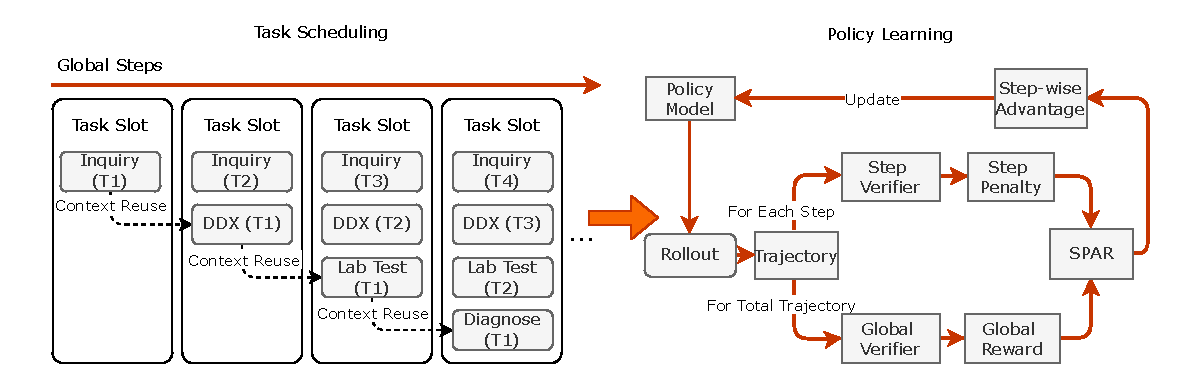
\includegraphics[width=0.98\linewidth]{image/osce.pdf}
    \caption{分段流水线 RL（左）与策略学习算法（右）。}
    \label{fig:spar}
\end{figure}


\subsection{深度临床问诊}
随着医疗 AI 的发展，“基于症状输入的即时诊断”需求迅速上升~\cite{liu2025medchainbridginggapllm}。然而，临床医学远不止简单知识检索，而是建立在严谨证据与演绎逻辑之上的学科。由于相同症状可能源于不同病因且患者个体风险阈值不同，可靠的临床决策必须依赖细粒度数据、系统化风险评估与可追溯推理~\cite{liao2020task, dou2024plpf}。

我们提出深度临床问诊框架，将问诊重新构想为临床级、结构化且可审计的信息生成过程。我们的目标是在简短交互内收集关键临床数据，同时保持严格安全标准。为此，我们提出一套训练框架（见图~\ref{fig:spar}），由分段流水线 RL 架构与带相对基线的逐步惩罚优势（SPAR）算法组成。


\subsubsection{分段流水线 RL}
我们将问诊表述为 $K$ 阶段的生成过程，取 $K=4$。令 $[K]=\{1,\dots,K\}$ 表示阶段索引，$\mathcal{S}=\{\text{Inq},\text{DDX},\text{Lab},\text{Diag}\}$ 为阶段类型集合。
对处于阶段 $k$ 的病例 $i$，用 $x_{k}^{(i)}$ 表示当前输入上下文，包含完整轨迹历史与本阶段指令（例如“基于以上内容，建议检验检查”）。策略 $\pi_\theta$ 生成响应片段 $y_{k}^{(i)}$：
\begin{equation}
    y_{k}^{(i)} \sim \pi_\theta(\cdot | x_{k}^{(i)})
\end{equation}
如图~\ref{fig:spar} 所示，我们采用异步多任务流水线：在全局步 $t$ 上，多个任务槽并行运行于不同流水线阶段（可对应不同病例）；这些阶段特定任务的并集构成训练批次 $\mathcal{B}_t$。

\paragraph{多任务训练目标。}
优化目标是相对于阶段特定目标提升生成片段 $y_k$ 的质量。对一批活跃上下文 $\mathcal{B}_t = \{x_{k_i}^{(i)}\}_{i=1}^N$，联合目标函数为：
\begin{equation}
    \mathcal{J}(\theta) = \frac{1}{|\mathcal{B}_t|} \sum_{x_{k}^{(i)} \in \mathcal{B}_t} \mathcal{L}_{\text{RL}} \left( y_{k}^{(i)}, \mathcal{G}_{k}^{(i)} \right)
\end{equation}
其中 $\mathcal{G}_k$ 为阶段 $k$ 的专属奖励函数。该表述将不同推理能力（信息收集与推导）统一到单一生成模型中。

\paragraph{基于门控迁移的上下文复用。}
流水线依赖自回归的上下文累积。下一阶段输入 $x_{k+1}^{(i)}$ 通过在当前上下文后拼接生成响应 $y_{k}^{(i)}$ 与下一阶段指令 $p_{k+1}$ 构建：
\begin{equation}
    x_{k+1}^{(i)} = [ x_{k}^{(i)}, y_{k}^{(i)}, p_{k+1} ]
\end{equation}
然而，开放式生成存在错误传播风险。为落实“输入垃圾则输出垃圾”的原则，我们实现质量门控迁移。下一阶段的训练池 $\mathcal{D}_{k+1}$ 通过过滤过程填充：
\begin{equation}
    \mathcal{D}_{k+1} \leftarrow 
    \begin{cases} 
        \mathcal{D}_{k+1} \cup \{ [ x_{k}^{(i)}, y_{k}^{(i)}, p_{k+1} ] \}, & \text{if } \mathcal{V}_{k}^{(i)} \ge \tau \\
        \mathcal{D}_{k+1}, & \text{otherwise (Discard)}
    \end{cases}
\end{equation}
其中 $\mathcal{V}_{k}^{(i)}$ 为阶段 $k$ 质量验证器给出的分数，$\tau$ 为接纳阈值。该机制保证只有具有临床有效逻辑链的轨迹被延展，从而有效从训练课程中剪除错误路径。

\subsubsection{策略学习算法：SPAR}
传统 RL 方法（如基于全局奖励的 GRPO~\cite{guo2025deepseek, DBLP:journals/corr/abs-2509-02333}）在长时程医学问诊中存在明显局限，包括奖励欺骗（通过重复提问抬高召回）、逻辑碎片化（临床转移断裂）以及归因无效。在长上下文对话中，轨迹级奖励难以隔离局部错误~\cite{zhang2025lets}，常导致训练不稳定，因为有效推理链会与局部缺陷一并被惩罚。

为解决这些问题，我们提出 SPAR（带相对基线的逐步惩罚优势），引入细粒度的逐步惩罚与解耦的优势估计机制，从而产生自适应课程学习效应。

\paragraph{奖励形式化。}
SPAR 采用层级奖励结构。对于由 $L$ 个逻辑交互步骤 $[z_1, \dots, z_L]$ 组成的生成回复 $y$，我们将每个步骤 $z_j$ 定义为一次完整的对话交换（即用户轮次后接助手轮次）。首先通过预定义临床量表（如诊断准确性、证据完整性）对整条轨迹评估，得到全局奖励 $R_{\text{global}}$。

同时，逐步验证器对每个交互步骤 $z_j$ 进行实时校验。令 $\mathbb{V}_j$ 表示由步骤 $z_j$ 触发的违规类型集合（如冗余、安全风险）。逐步有效性系数 $\gamma_j \in (0, 1]$ 定义为：
\begin{equation}
    \gamma_j =
    \begin{cases}
        1, & \text{if } \mathbb{V}_j = \emptyset \\
        \min\limits_{v \in \mathbb{V}_j} (\lambda_v), & \text{otherwise}
    \end{cases}
\end{equation}
其中 $\lambda_v \in (0, 1)$ 为违规类型 $v$ 的惩罚系数。该形式化遵循最小有效性原则：若某一步出现多种错误，仅施加最严重惩罚（最小 $\lambda$）。该步的有效回报为 $R_j = \gamma_j \cdot R_{\text{global}}$。


\paragraph{逐步优势估计。}
SPAR 的核心创新在于优势计算，将局部惩罚与组内基线解耦。与使用惩罚后分布归一化奖励的传统方法不同，SPAR 通过将\textit{逐步惩罚回报}与\textit{未惩罚组均值}比较来计算步骤 $z_j$ 的优势 $\hat{A}_{j}$：
\begin{equation}
    \hat{A}_{j} = \frac{\gamma_{j} R_{\text{global}} - \mu_{\text{raw}}}{\sigma_{\text{raw}} + \epsilon}
\end{equation}
其中 $\mu_{\text{raw}}$ 与 $\sigma_{\text{raw}}$ 分别为采样组内原始全局奖励（$R_{\text{global}}$）的均值与标准差，不包含任何逐步惩罚。此处采样组指在同一提示（即相同问诊上下文）下生成的多条 rollout，从而支持候选之间的相对比较。

随后我们采用 GSPO 风格的策略更新~\cite{DBLP:journals/corr/abs-2507-18071}，使用逐步优势 $\hat{A}_j$ 加权似然比目标，使惩罚归因于触发违规的具体交互步骤。此处采样组指在同一提示（即相同问诊上下文）下生成的多条 rollout，从而支持候选之间的相对比较。

% We then apply a GSPO-style policy update~\cite{DBLP:journals/corr/abs-2507-18071}, using the step-wise advantages $\hat{A}_j$ to weight the likelihood-ratio objective, so that penalties are attributed to the specific interaction steps responsible for violations.

\paragraph{隐式课程机制。}
该优势设计通过根据错误严重程度自然调度优化优先级，从而形成隐式课程~\cite{bengio2009curriculum}：
\begin{itemize}
    \item \textbf{阶段 1：纠正关键错误。} 对严重违规（如重复），施加严格惩罚（如 $\lambda \approx 0.1$）。这将有效回报 $\gamma_j R_{\text{global}}$ 拉低到显著低于组基线 $\mu_{\text{raw}}$，产生强烈负优势（$\hat{A}_j \ll 0$）。该主导梯度信号促使模型在训练早期优先修复基础可用性问题。
    \item \textbf{阶段 2：细节打磨。} 对轻微瑕疵（如措辞僵硬）采用较轻惩罚（如 $\lambda \approx 0.9$）。初期该微小偏差被全局奖励的高方差（$\sigma_{\text{raw}}$）掩盖；随着策略稳定、$\sigma_{\text{raw}}$ 下降，这些细粒度信号开始主导梯度方向，引导模型向表达质量优化。
\end{itemize}
通过隔离特定步级行为的影响，SPAR 实现精细的归因，将局部缺陷与总体诊断成功区分开来。


\subsection{可信健康咨询}
% 孙
% 可信临床决策
% 临床一致性咨询
本节详细介绍我们面向可信健康咨询的训练方法，聚焦临床可信度与交互效用的融合。为克服静态反馈的局限，我们首先引入动态量表演化框架，以缓解奖励欺骗并确保模型追求真实推理而非表层模式。随后，我们提出事实感知强化学习策略以增强模型的事实推理能力。该方法超越朴素惩罚机制，既能有效抑制不忠实幻觉，又避免诱发保守倾向，从而保持模型提供细致且有信息量的医学建议能力。

\subsubsection{动态量表演化}
在先前工作~\cite{baichuan-m2} 中，我们提出了基于量表的 RL 以提升临床推理能力。但我们观察到该方法容易遭受“奖励欺骗”。模型倾向于追求表层的“高分表现”而非真实推理，表现为被动冗长、模板化防御或臆造细节。其根因在于以往量表仅依赖\textit{输入问题}构建；问题固定后量表静态化，形成可被模型轻易利用的可预测结构。

为解决该问题，我们在 M3 中显著升级反馈信号质量。受 \cite{DBLP:journals/corr/abs-2511-19399,DBLP:journals/corr/abs-2509-21500} 启发，我们提出人机协同的动态演化机制，在量表合成过程中关键性地纳入\textit{模型的响应}。具体而言，我们将约束分为两类：

\begin{itemize}
    \item \textbf{核心量表集合：} 仅基于问题合成，用于引导模型优化总体方向并保证基础安全。
    \item \textbf{动态量表集合：} 基于问题\textit{与}模型历史响应动态合成，用于约束训练过程中发现的不合规行为与具体脆弱点。
\end{itemize}
该动态集合的构建与维护依赖两个关键模块：质量控制与准入/退出规则。

\paragraph{质量控制}
为确保动态生成量表的有效性与临床相关性，我们实现“挖掘-验证-注入”的闭环流程。
首先识别高置信样本——在当前系统下得分高但潜藏缺陷的响应。
随后量表挖掘代理分析这些样本，识别对抗模式并拟定候选约束。
最后由人类专家进行校验。专家无需从零制定规则，而是审核代理输出，评估其边界确定性与元原则一致性（如安全性 $>$ 经验性）。这确保量表激励推理本身，而非转移奖励欺骗的焦点。

\paragraph{准入与退出规则}
为防止规则爆炸并保持奖励信号强度，动态量表集合遵循“问题驱动”的生命周期：

\begin{itemize}
    \item \textbf{准入：} 候选量表并非仅因“正确”而被接纳，只有当其针对统计显著的失败模式（即模型响应中违规率较高）时才会激活，从而保证反馈聚焦于活跃行为缺陷。
    \item \textbf{退出：} 当某约束在多个训练轮次中持续被满足（违规率 $\rightarrow 0$）时，将自动从动态集合中移除。该“剪枝”机制防止奖励信号被稀释，使优化焦点严格聚焦于新出现且未解决的问题，而不被冗余正向奖励冲淡。
\end{itemize}


\subsubsection{事实感知强化学习}
\label{sec:fact-aware}

在带验证奖励的强化学习（RLVR）范式中，朴素的幻觉抑制策略通常将验证信号直接转化为标量惩罚~\cite{DBLP:conf/emnlp/MinKLLYKIZH23, chen2025learning}。标准目标形式定义为：
\begin{equation}
R = R_{task} + \alpha \cdot R_{hallu}
\label{eq:naive-objective}
\end{equation}
其中 $R_{hallu}$ 使用基于计数的幻觉率度量（$-N_{\text{hallu}}/N_{\text{total}}$）。该目标试图在惩罚项降低幻觉的同时保留核心医学推理能力（$R_{task}$），但在长文本生成中容易遭受两种主要的奖励欺骗：

\begin{itemize}
    \item \textbf{冗余稀释：} 模型通过生成大量事实正确但价值较低的陈述来抬高分母 $N_{\text{total}}$，在不修正核心错误的情况下降低测得的幻觉率。

    \item \textbf{惩罚诱导的保守：} 严苛惩罚会促使模型采取过度保守策略（如缩短输出以规避惩罚），从而削弱探索与复杂推理行为的习得。
\end{itemize}
为解决这些问题，我们提出包含结构化信号去噪与动态多目标聚合的联合优化框架，如图~\ref{fig:fact_aware_rl_fig} 所示。

\begin{figure}[t]
    \centering
    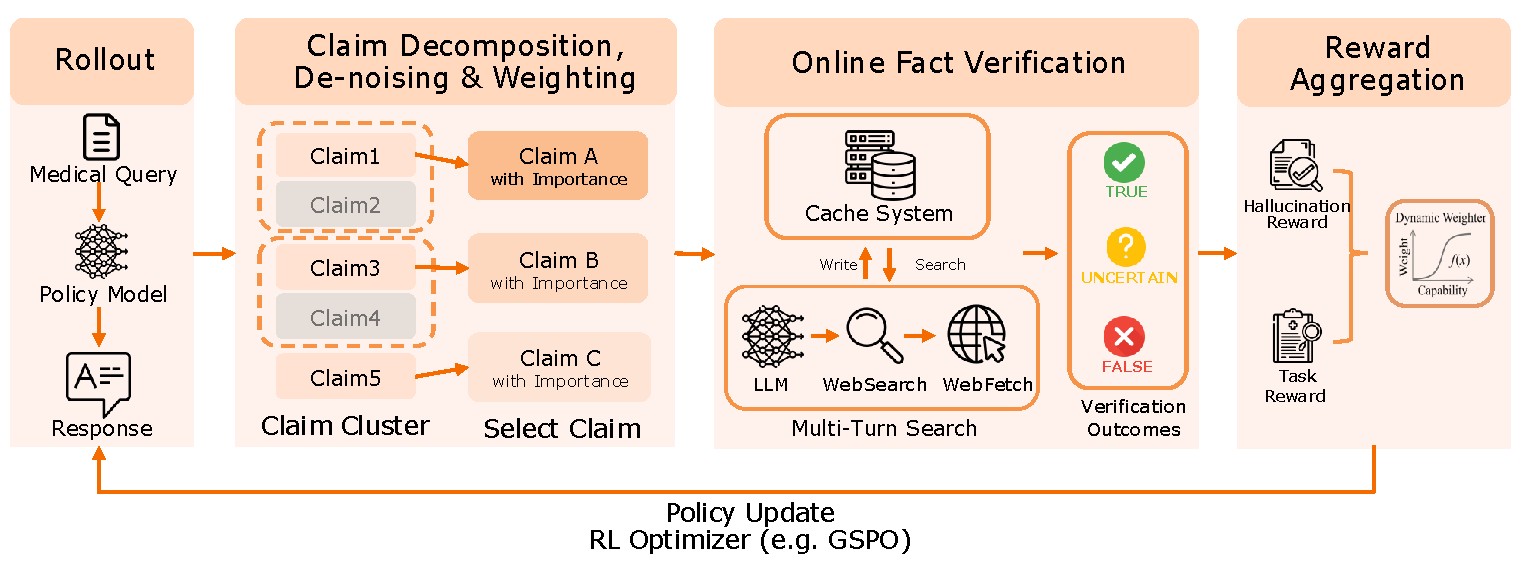
\includegraphics[width=0.98\linewidth]{image/fact-aware-rl.pdf}
    \caption{事实感知强化学习算法。}
    \label{fig:fact_aware_rl_fig}
\end{figure}

\paragraph{结构化信号去噪}

为建立对冗余鲁棒的奖励信号，我们将原子事实的验证重构为基于语义密度的加权评估，确保核心诊断陈述中的幻觉受到显著高于边缘内容的惩罚。

我们首先通过语义编码器 $\mathcal{E}(\cdot)$ 将回复序列 $\{s_j\}$ 与抽取事实 $\{c_i\}$ 映射到向量空间。为防止通过同义改写操纵指标，我们使用余弦相似度阈值进行语义聚类。对每个簇 $\mathcal{C}_k$ 选取代表事实 $c_k^*$，将评估指标从词频转为语义单元密度。随后用显著性权重 $w(c_k^*)$ 量化每条事实的信息贡献，定义为其在回复句子中的最大语义相关性：
\begin{equation}
w(c_k^*) = \max_{1 \le j \le M} \cos(\mathcal{E}_{c_k^*}, \mathcal{E}_{s_j})
\end{equation}
事实性奖励 $R_{fact}$ 计算为加权惩罚项：
\begin{equation}
R_{fact} = - \frac{\sum_{k=1}^{K} w(c_k^*) \cdot \mathbb{I}(c_k^*)}{\sum_{k=1}^{K} w(c_k^*) + \epsilon}
\end{equation}
其中 $\mathbb{I}(c_k^*)$ 为验证惩罚指示函数，定义为：
\begin{equation}
\mathbb{I}(c_k^*) = 
\begin{cases} 
1 & \text{if } c_k^* \in \{\text{Refuted}, \text{Uncertain}\} \\
0 & \text{otherwise}
\end{cases}
\end{equation}
从机制上看，加权分母抵消事实数量膨胀（抗稀释），而依赖显著性的分子确保惩罚集中于核心错误而非边缘文本，从而保留推理效用。

\paragraph{动态多目标聚合}

为平衡医学推理强化与幻觉抑制，我们实现动态聚合机制，引入软门控系数 $\lambda(R_{task})$，根据在策略生成回复上获得的任务奖励调节惩罚强度。

给定特定回复的 $R_{task}$，我们使用成形 Sigmoid 函数将动态系数 $\lambda(R_{task})$ 严格定义为任务奖励的函数：
\begin{equation}
\lambda(R_{task}) = \sigma \left( \kappa \cdot \frac{R_{task} - \mu}{\Delta} \right)
\end{equation}
其中 $\sigma(\cdot)$ 为标准 sigmoid 函数，中心为 $\mu = (\tau_{min} + \tau_{max})/2$，尺度为 $\Delta = \tau_{max} - \tau_{min}$（陡峭度 $\kappa=10$）。

阈值通过对任务奖励分布的后验分析进行校准。我们设定 $\tau_{min} = 0.75$、$\tau_{max} = 0.95$ 以界定反映有效医学推理的关键区间，使惩罚强度与模型能力相匹配：

\begin{itemize}
    \item \textbf{保护区（$R_{task} < \tau_{min}$）：} $\lambda(R_{task}) \to 0$。抑制惩罚以优先优化能力，避免干扰基础推理技能的习得。
    \item \textbf{过渡区（$\tau_{min} \le R_{task} \le \tau_{max}$）：} $\lambda(R_{task})$ 非线性上升，系统逐步引入事实约束。
    \item \textbf{约束区（$R_{task} > \tau_{max}$）：} $\lambda(R_{task}) \to 1$。当模型具备足够推理能力时施加完整惩罚，以最大化幻觉抑制。
\end{itemize}

最终总奖励 $R$ 将任务效用与门控事实惩罚项聚合：
\begin{equation}
R = R_{task} + \lambda(R_{task}) \cdot R_{fact}
\label{eq:full-fact-aware-rl}
\end{equation}
该形式化实现了隐式课程：先保障推理能力，再施加严格安全约束。我们在附录 \ref{sec:ablation_reward} 中通过对比消融实验验证这一行为。

















% \subsection{Other Reasoning Tasks}

% yangfan: 这部分在正文中不重点介绍，medxqa-rubrics 可以在附录中说明
% 需要补充一个实验：纯 RLVR（answer verify） 的 baseline。
% This section introduces the training for Medical QA tasks. 
% MedBullet, M2 General Task
% GRPO, RLVR


\section{评测}
为全面评估 Baichuan-M3 的临床效用与安全性，我们在两个互补维度上进行严格实验：动态临床流程模拟（\textbf{ScanBench}）与广谱医学推理（\textbf{HealthBench}~\cite{healthbench}）。我们将 Baichuan-M3 与多种有竞争力的基线进行对比，以确保评估的稳健性。这些基线包括推理能力突出的通用大模型（如 \textbf{GPT-5.2-High}\cite{openai2025gpt52}、\textbf{Deepseek-V3.2-Thinking}\cite{deepseek2025v32thinking}、\textbf{Qwen3-235B-thinking-2507}\cite{qwen3-235b-thinking-2507}）、代表性的医疗专用模型（如 \textbf{AntAngelMed}\cite{antangelmed2026}）以及上一代模型（\textbf{Baichuan-M2}~\cite{baichuan-m2}）。关键的是，为与真实专业标准对齐，我们引入由三甲医院主治医师组成的人类基线，每位医生至少具有 5 年临床经验。该对比分析旨在验证模型在复杂决策、专业知识应用与幻觉抑制方面相较通用大模型、领域模型与人类专家的进步。

\subsection{ScanBench}
不同于传统静态问答基准，ScanBench 模拟真实临床流程“问诊 $\rightarrow$ 检验检查 $\rightarrow$ 诊断”。该数据集计划开源，将多样临床病例转化为可观测、可量化的决策路径，并划分为三个渐进阶段。

\subsubsection{数据集构成与统计}
ScanBench 从病例多样性、问诊粒度与检查复杂度三个维度高保真地模拟真实临床环境。

\paragraph{临床病例多样性}
如表~\ref{tab:scanbench_distribution} 所示，ScanBench 包含来自 12 个科室的 303 个病例，覆盖常见疾病（如全科）与长尾专科（如风湿科、血液科）。

\begin{table}[H]
\centering
\caption{按科室划分的临床样本分布。}
\label{tab:scanbench_distribution}
\begin{tabular}{lclc} % Compacted the table slightly
\toprule
\textbf{Department} & \textbf{Count} & \textbf{Department} & \textbf{Count} \\ \midrule
General Practice    & 111 & Nephrology           & 15 \\
Surgery             & 50  & Cardiology           & 14 \\
Gynecology          & 26  & Respiratory Medicine & 14 \\
Neurology           & 25  & Endocrinology        & 7  \\
Gastroenterology    & 18  & Rheumatology         & 6  \\
Hematology          & 15  & Geriatrics           & 2  \\ \bottomrule
\end{tabular}
\end{table}

\paragraph{问诊粒度与严谨性}
为量化问诊过程，我们标注了 8,857 条清单项作为真值。
\begin{itemize}
    \item \textbf{信息密度：} 每个病例平均包含 29.23 项（范围：20--35），需要持续的多轮上下文跟踪。
    \item \textbf{逻辑分布：} 清单反映临床诊断逻辑：现病史占比最高（55.8\%），其次为既往史（19.6\%）与个人/社会史（14.6\%），并在相关时包含产科/妇科史（5.4\%）与家族史（4.7\%）。
    \item \textbf{关键性权重：} 我们区分关键安全要点与一般信息：51.3\% 标注为 Level 2（关键），用于诊断与风险排除，其余 48.7\% 为 Level 1（补充）。
\end{itemize}

\paragraph{综合检查动作空间}
在辅助检查阶段，模型在 38 个类别的统一动作空间内进行选择，模拟真实医院的资源管理复杂度，包括：
\begin{itemize}
    \item \textbf{常规与生化：} 血/尿/便常规、肝肾功能、电解质、CRP、糖代谢（含 OGTT/HbA1c）等。
    \item \textbf{影像与功能：} CT、MRI、超声、X 光、心电图、脑电图、肺功能等。
    \item \textbf{病理与专科：} 肿瘤标志物、病毒标志物、自身抗体、激素、骨髓活检、内镜等。
\end{itemize}
这一丰富的候选集要求模型在避免资源浪费的同时精准选择必要检查。

\subsubsection{流程与评估方法}
评估流程始于站点 1：问诊，模型与标准化病人进行多轮互动。为评估过程质量，我们引入 SCAN 框架，将问诊表现分解为四个维度：风险分层（Safety Stratification）、信息澄清（Information Clarification）、关联性提问（Associative Questioning）与规范化输出（Normative Output）。我们使用 GPT-4.1~\cite{gpt4} 验证 OSCE 关键临床要点的覆盖度，同时剔除每次问诊中反复出现且非诊断性的内容（如反复陈述年龄/性别或模板化自我介绍）。

% Given the elicited evidence, Station 2: Lab Testing evaluates both resource efficiency and interpretative accuracy. The model proposes a differential diagnosis and selects laboratory or imaging tests from a unified candidate pool. Performance is measured by F1 against a physician-curated ground-truth set, reflecting the trade-off between ordering precision and recall.

在已获得证据的基础上，站点 2：检验检查评估资源效率与解读准确性。模型提出鉴别诊断并从统一候选池中选择检验或影像检查，候选检查根据对诊断与决策的贡献被划分为“必需”与“可选”。性能采用加权 F1 评估，其中对必需检查的召回赋予更高权重，以体现其在诊断流程中的重要性，同时保持整体精确率与覆盖率的平衡评价。

流程在站点 3：诊断结束，模型整合所有先验信息做出最终诊断。我们采用基于 ICD-10 分类的层级匹配标准：正确命中叶子节点得到奖励，分支偏离则受到惩罚。


\subsubsection{性能分析}

如图~\ref{fig:scan_bench_main} 所示，Baichuan-M3 在三大站点均排名第一，展现出全面优势。尤其在最具挑战的临床问诊阶段，得分 74.9，较第二名 GPT-5.2-High 高出 12.4 分，并超过人类基线 20 分以上。这一优势同样体现在检验检查（72.1）与最终诊断（74.4）上，表明 Baichuan-M3 具备稳健的端到端医学推理能力，而非仅在孤立任务上表现突出。

\begin{figure}[H]
    \centering
    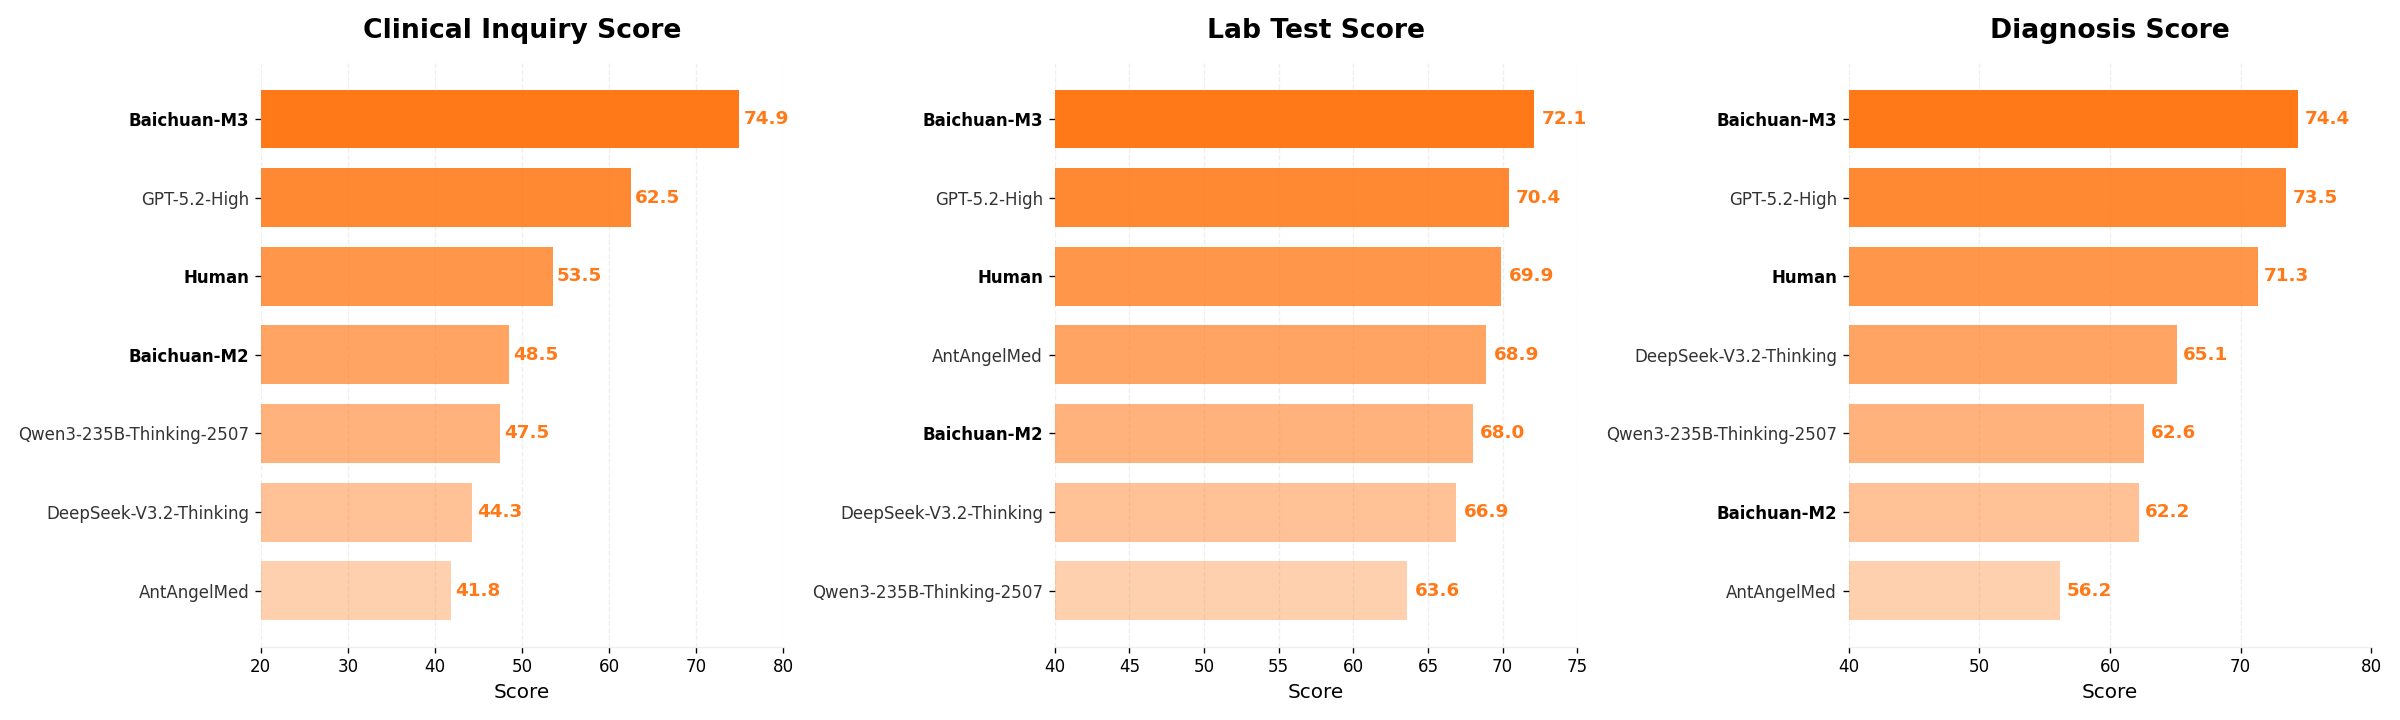
\includegraphics[width=1.0\linewidth]{image/scan_1x3.png}
    \caption{ScanBench 总体性能对比。}
    \label{fig:scan_bench_main}
\end{figure}


使用 SCAN 框架对问诊能力进行进一步拆解（图~\ref{fig:scan_bench_dims}），Baichuan-M3 是唯一在四个维度上均展现显著领先的模型，持续超越 SOTA 大模型与人类专家。

具体而言，在风险分层方面，Baichuan-M3 取得 75.8 的高分，显著领先第二名 Qwen3-235B（48.3），几乎是人类基线（40.1）的两倍。这表明其对“红旗”症状与关键风险具有更高敏感性。在关联性提问方面，得分 72.6，显著超过 GPT-5.2-High（54.5），体现其对鉴别诊断的精细把握，能够主动挖掘超越用户初始描述的潜在线索。此外，Baichuan-M3 在清晰度（84.5）与规范化流程（59.9）上表现突出，保证收集信息既细致又结构化标准化。综合这些优势，Baichuan-M3 构建了精确问诊与安全决策的闭环，标准化水平超过人类基线。

\begin{figure}[H]
    \centering
    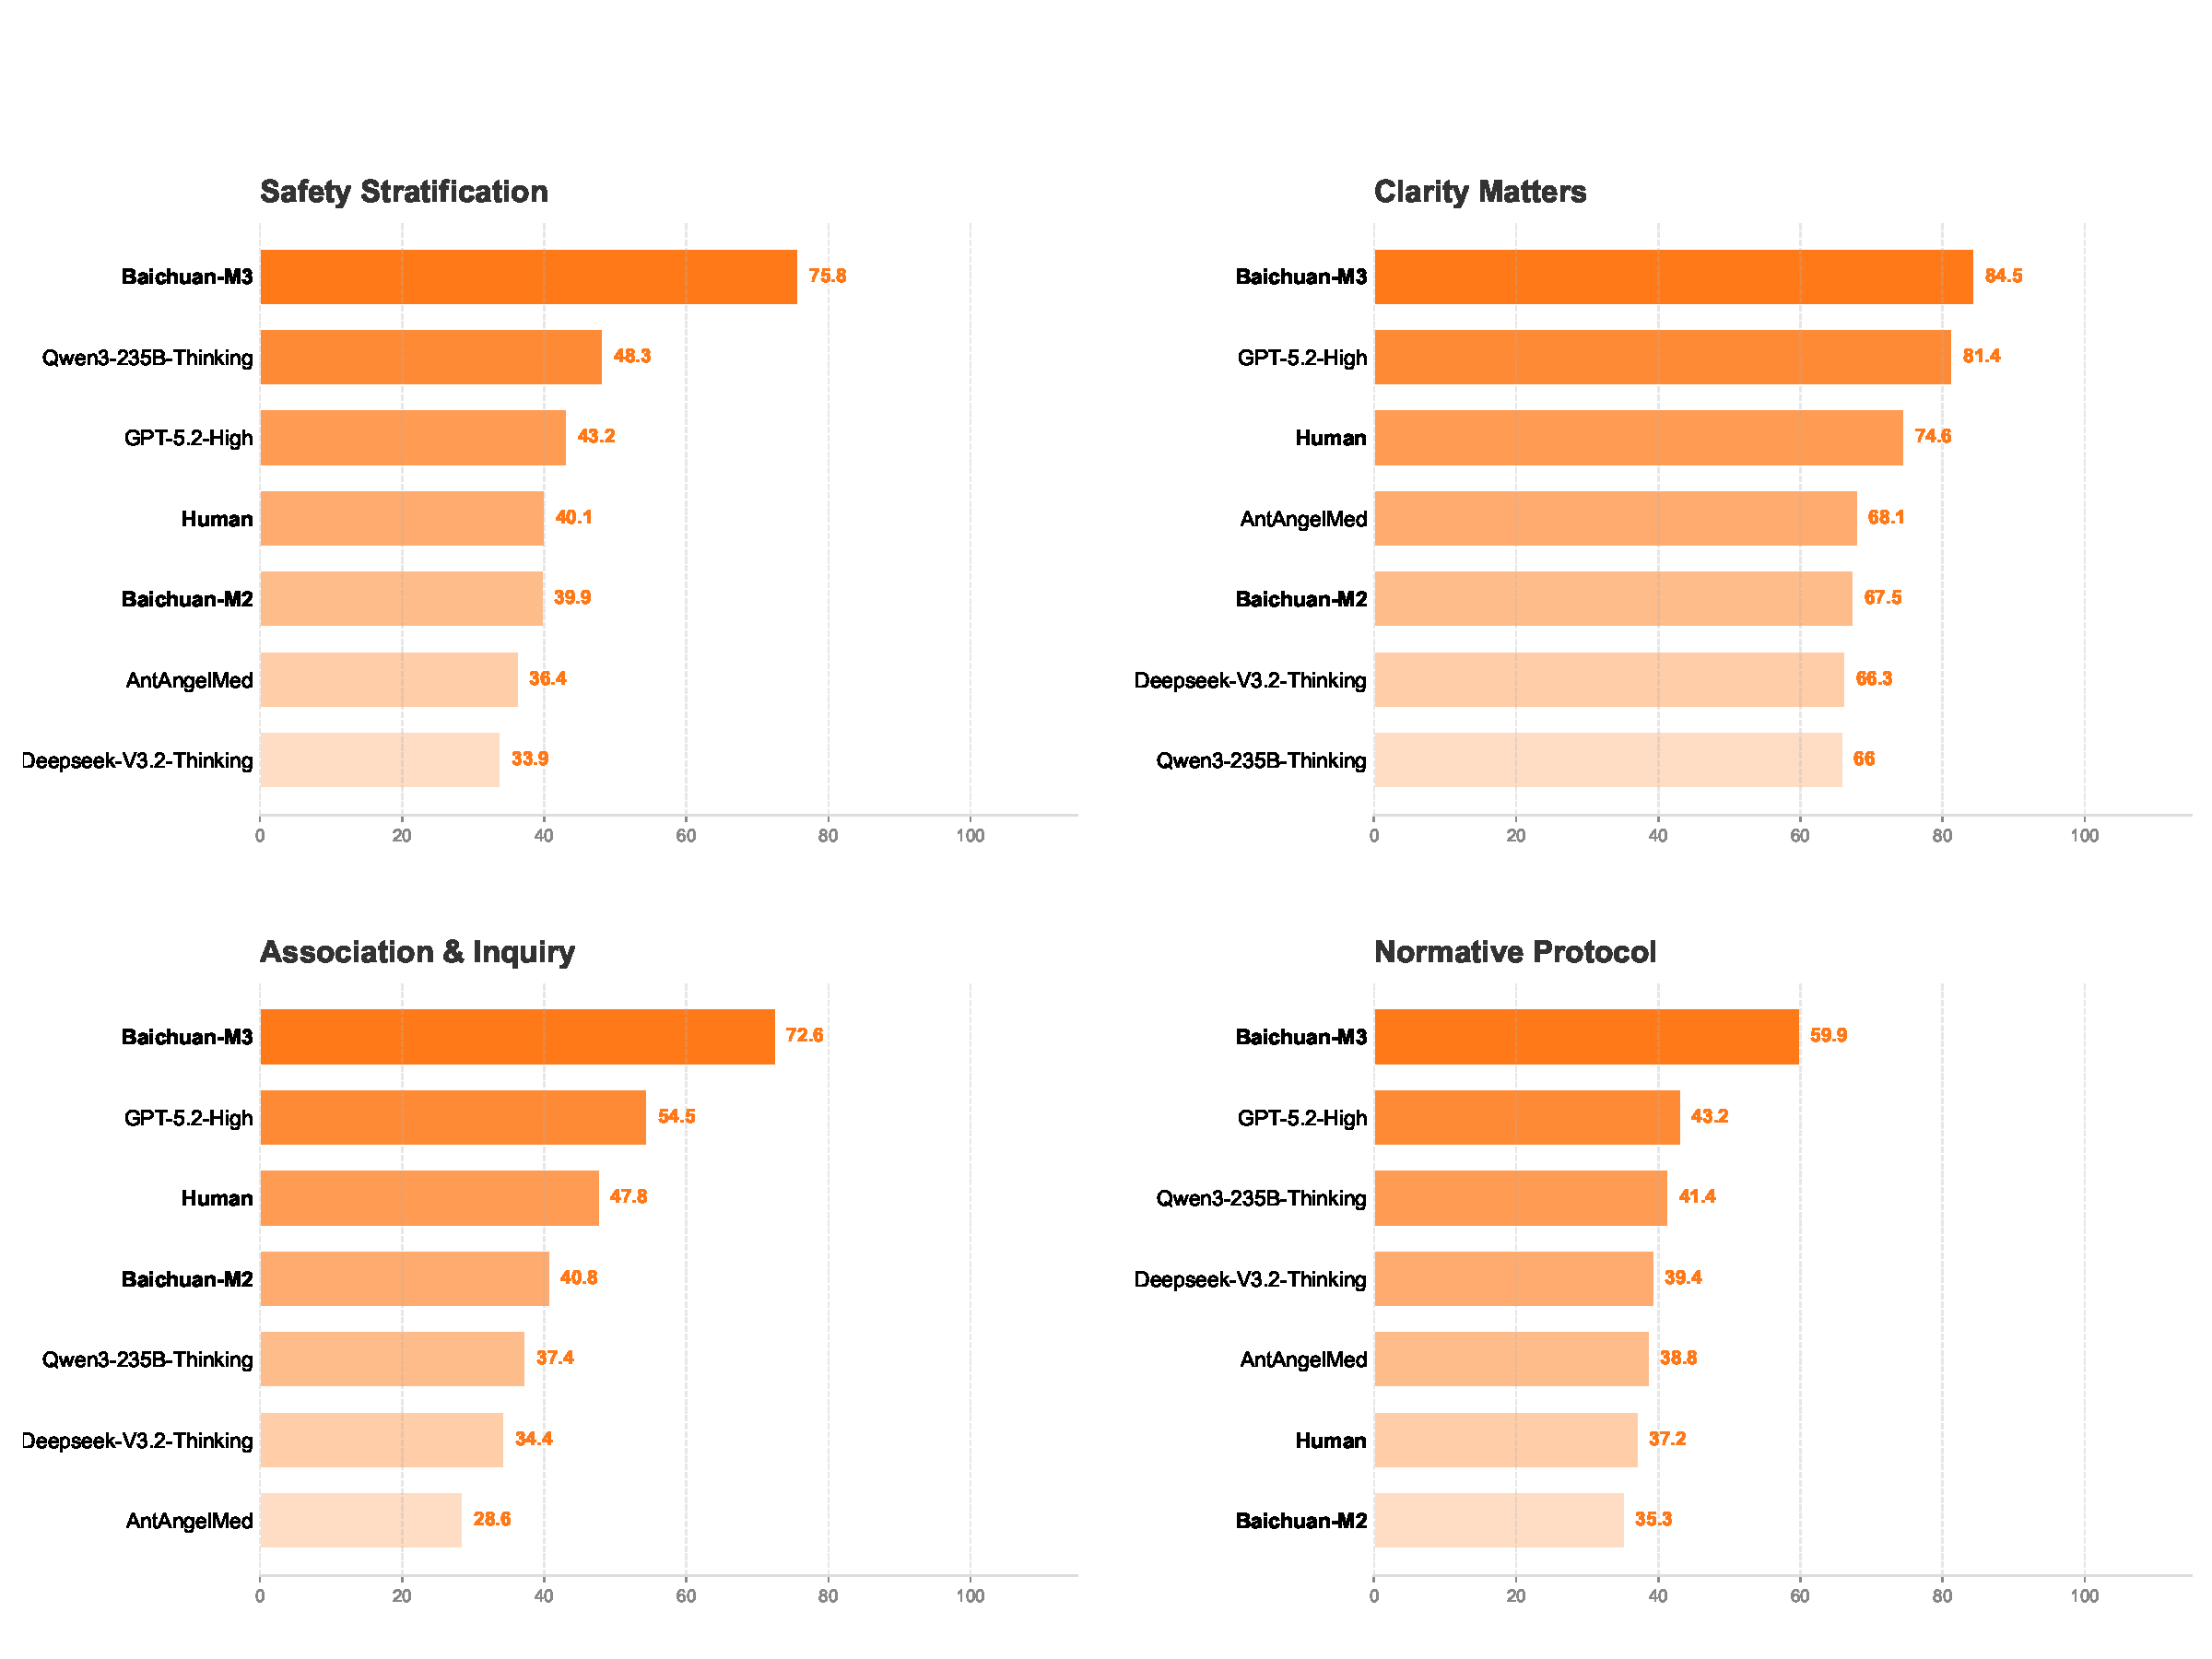
\includegraphics[width=1.0\linewidth]{image/scan_2x2.pdf}
    \caption{问诊能力的细粒度拆解。}
    \label{fig:scan_bench_dims}
\end{figure}


\subsubsection{动态问诊效率}
图~\ref{fig:scan_turn_evlo} 展示了模型分数随对话轮次变化的趋势。为减少极少数超长对话带来的噪声，我们剔除样本占比低于 10\% 的轮次区间，使趋势更易解读。


\paragraph{基础收敛，推理分化}
图~\ref{fig:scan_turn_evlo}b 显示，大多数模型在症状澄清上很快达到相近水平（约 0.7--0.8）。差距在关联性提问上逐渐显现（图~\ref{fig:scan_turn_evlo}c）：Baichuan-M3 随对话推进持续提升，而通用模型（如 Deepseek 与 Qwen）逐渐落后——在长时程场景形成近乎两倍的优势。

\paragraph{风险敏感性与上下文遵循}
在风险分层方面（图~\ref{fig:scan_turn_evlo}a），Baichuan-M3 对风险信号更敏感，随证据累积得分上升至约 0.7。相比之下，GPT-5.2-High 即使在较长对话中也徘徊在 0.5 左右，显示急性风险识别能力较弱。在规范化流程方面（图~\ref{fig:scan_turn_evlo}d），模型表现随轮次提升而提高，表明保持上下文有助于遵循结构化临床流程。

\begin{figure}[H]
    \centering
    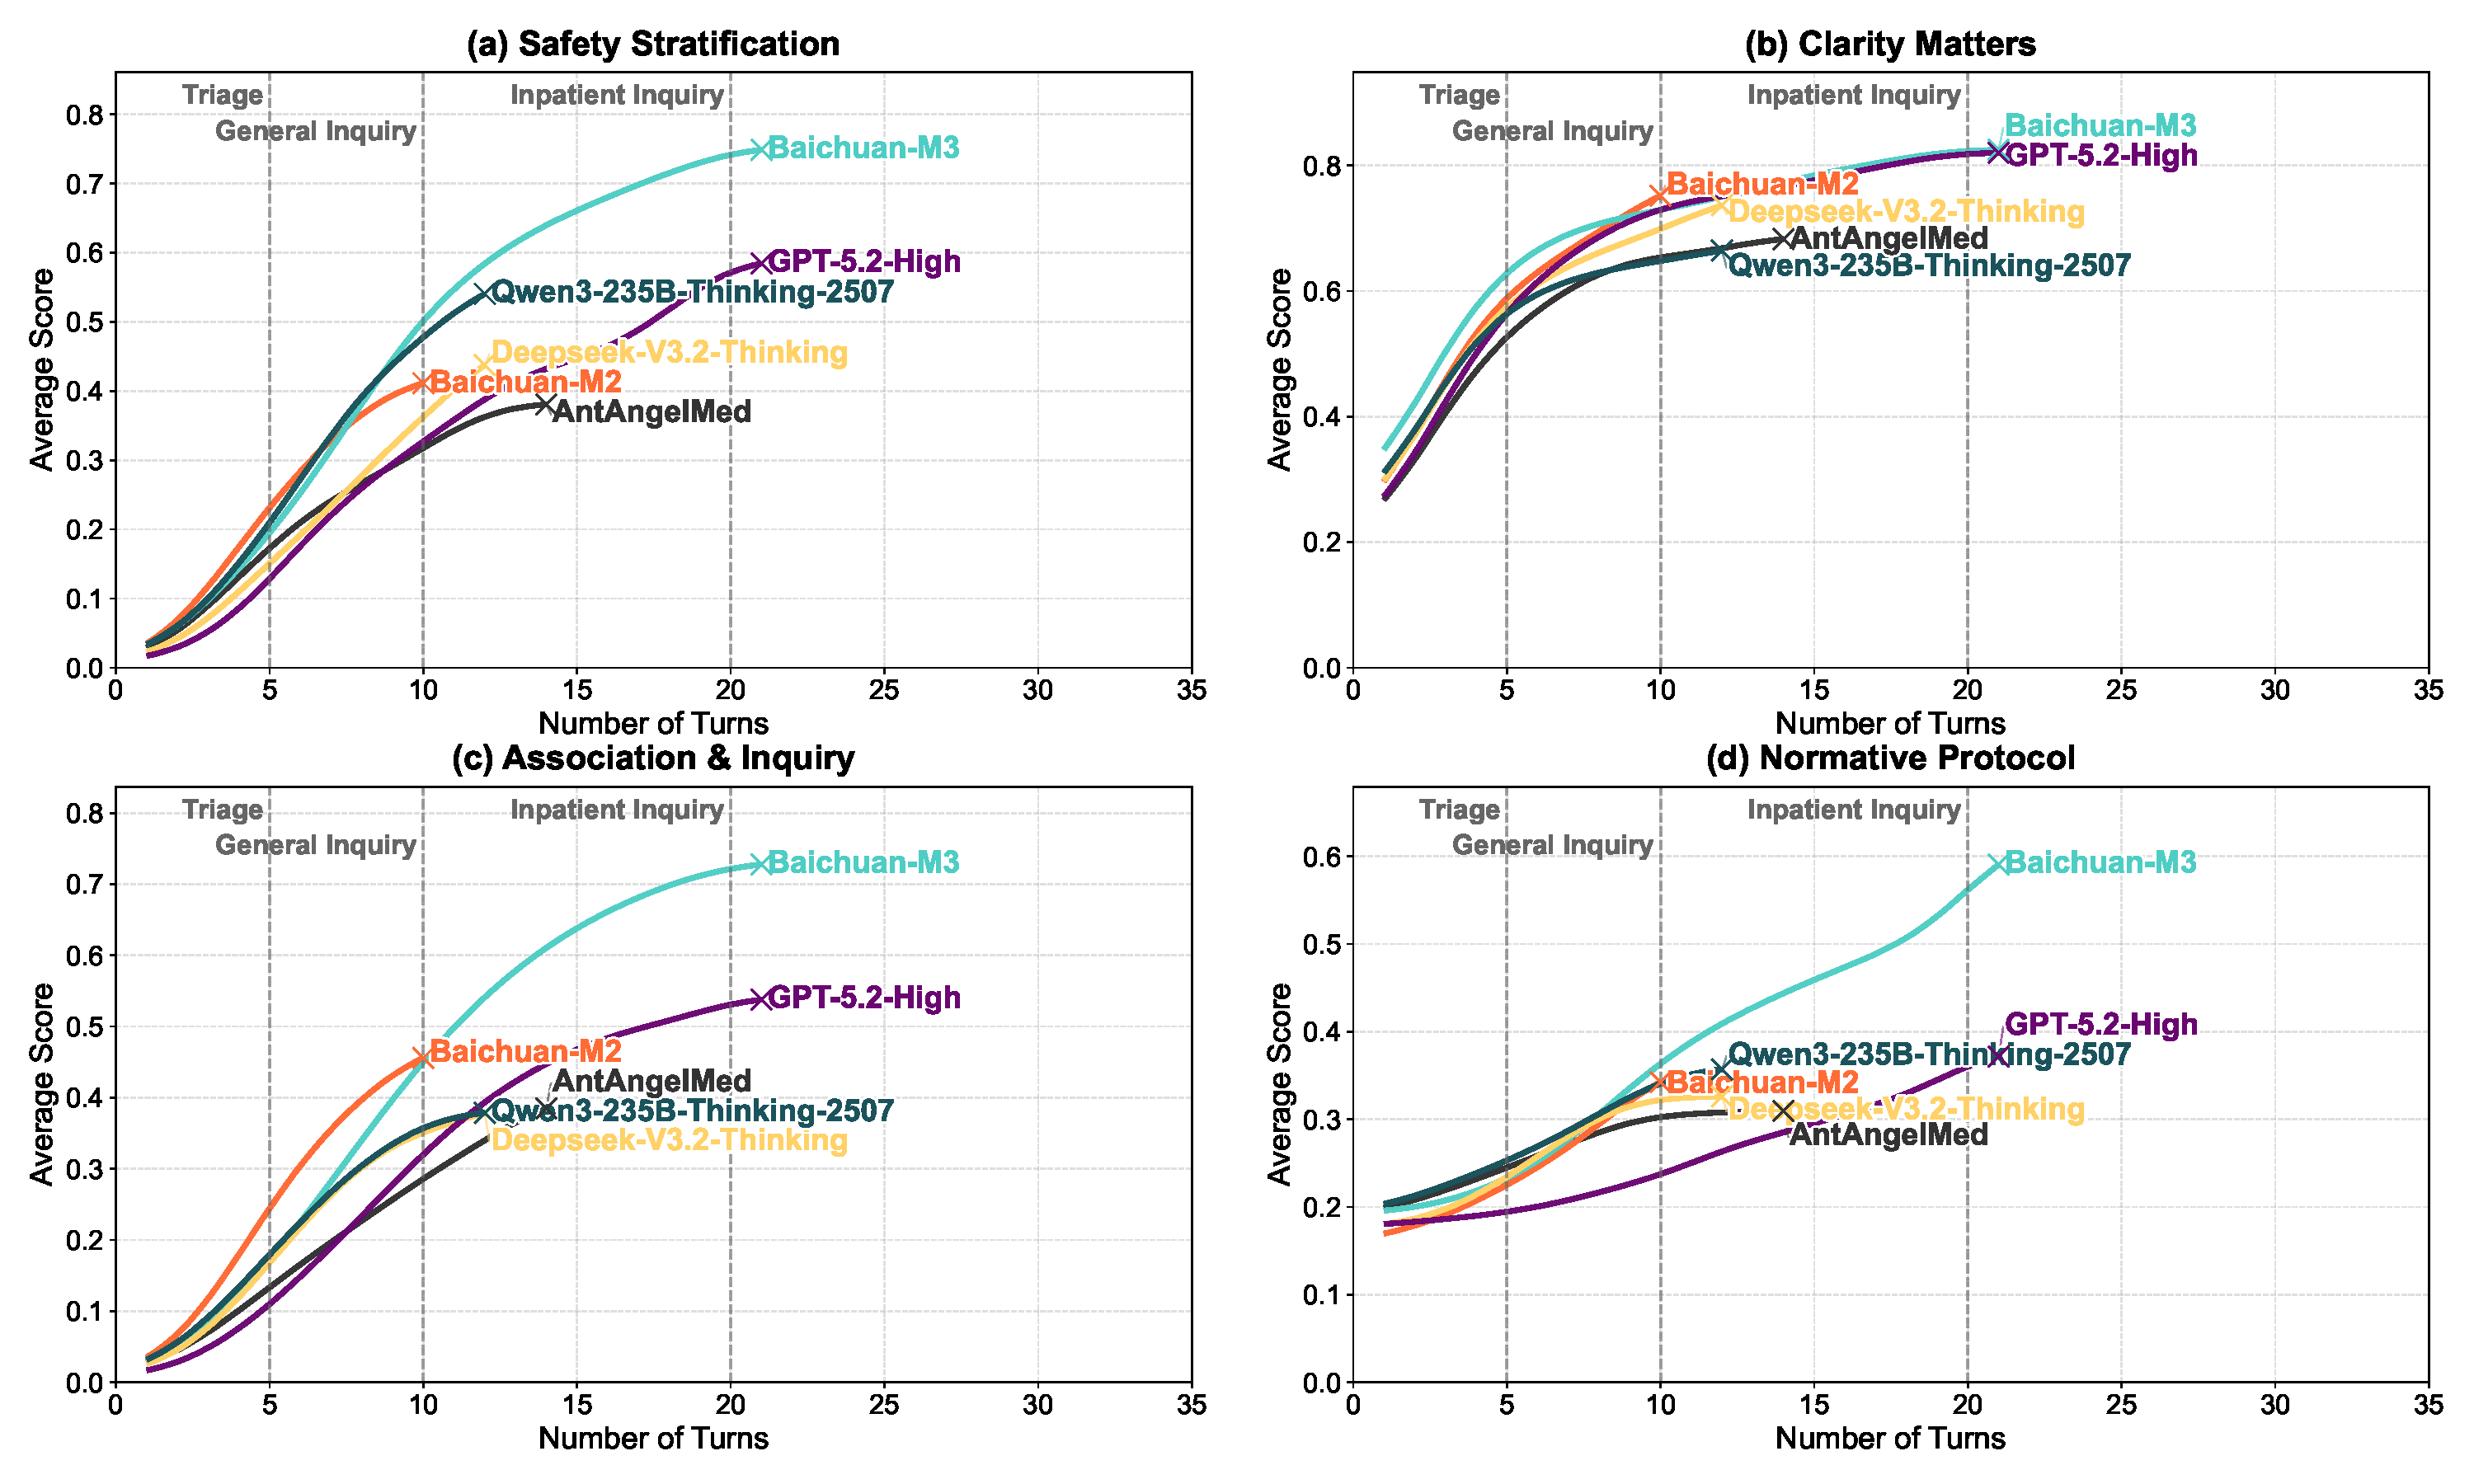
\includegraphics[width=0.95\linewidth]{image/merged_metrics_SCAN.pdf}
    \caption{模型性能随对话轮次的演化。}
    \label{fig:scan_turn_evlo}
\end{figure}


总之，通用 LLM 可满足基础信息采集，但临床场景所需的复杂推理与安全保障仍离不开专门训练。


\subsection{HealthBench}
% 1. 引言部分：只介绍 Bench 本身
HealthBench 是评估 LLM 临床推理能力与安全边界的严格基准。通过在不同难度与维度上评估性能，它提供了模型在真实医疗场景中效用的全面视角。

\subsubsection{HealthBench-Main}
% 2. 第一段：Overall Performance (SOTA 对比)
如图~\ref{fig:exp_hb} 所示，\textbf{Baichuan-M3} 在所有关键指标上建立了新的 SOTA 标准。在综合 \textit{HealthBench Total} 上，Baichuan-M3 得分 \textbf{65.1}，明显超过亚军 GPT-5.2-High（63.3）。在高难度 \textit{HealthBench Hard} 子集上，Baichuan-M3 进一步扩大领先优势，得分 \textbf{44.4}，显著超过 GPT-5.2-High（42.0）与 AntAngelMed（39.6）。此外，Baichuan-M3 以 \textbf{3.5\%} 的最低\textit{幻觉率}展现出卓越可靠性，表明其在深度临床推理与事实准确性之间取得了更稳健的平衡。

\begin{figure}[H]
    \centering
    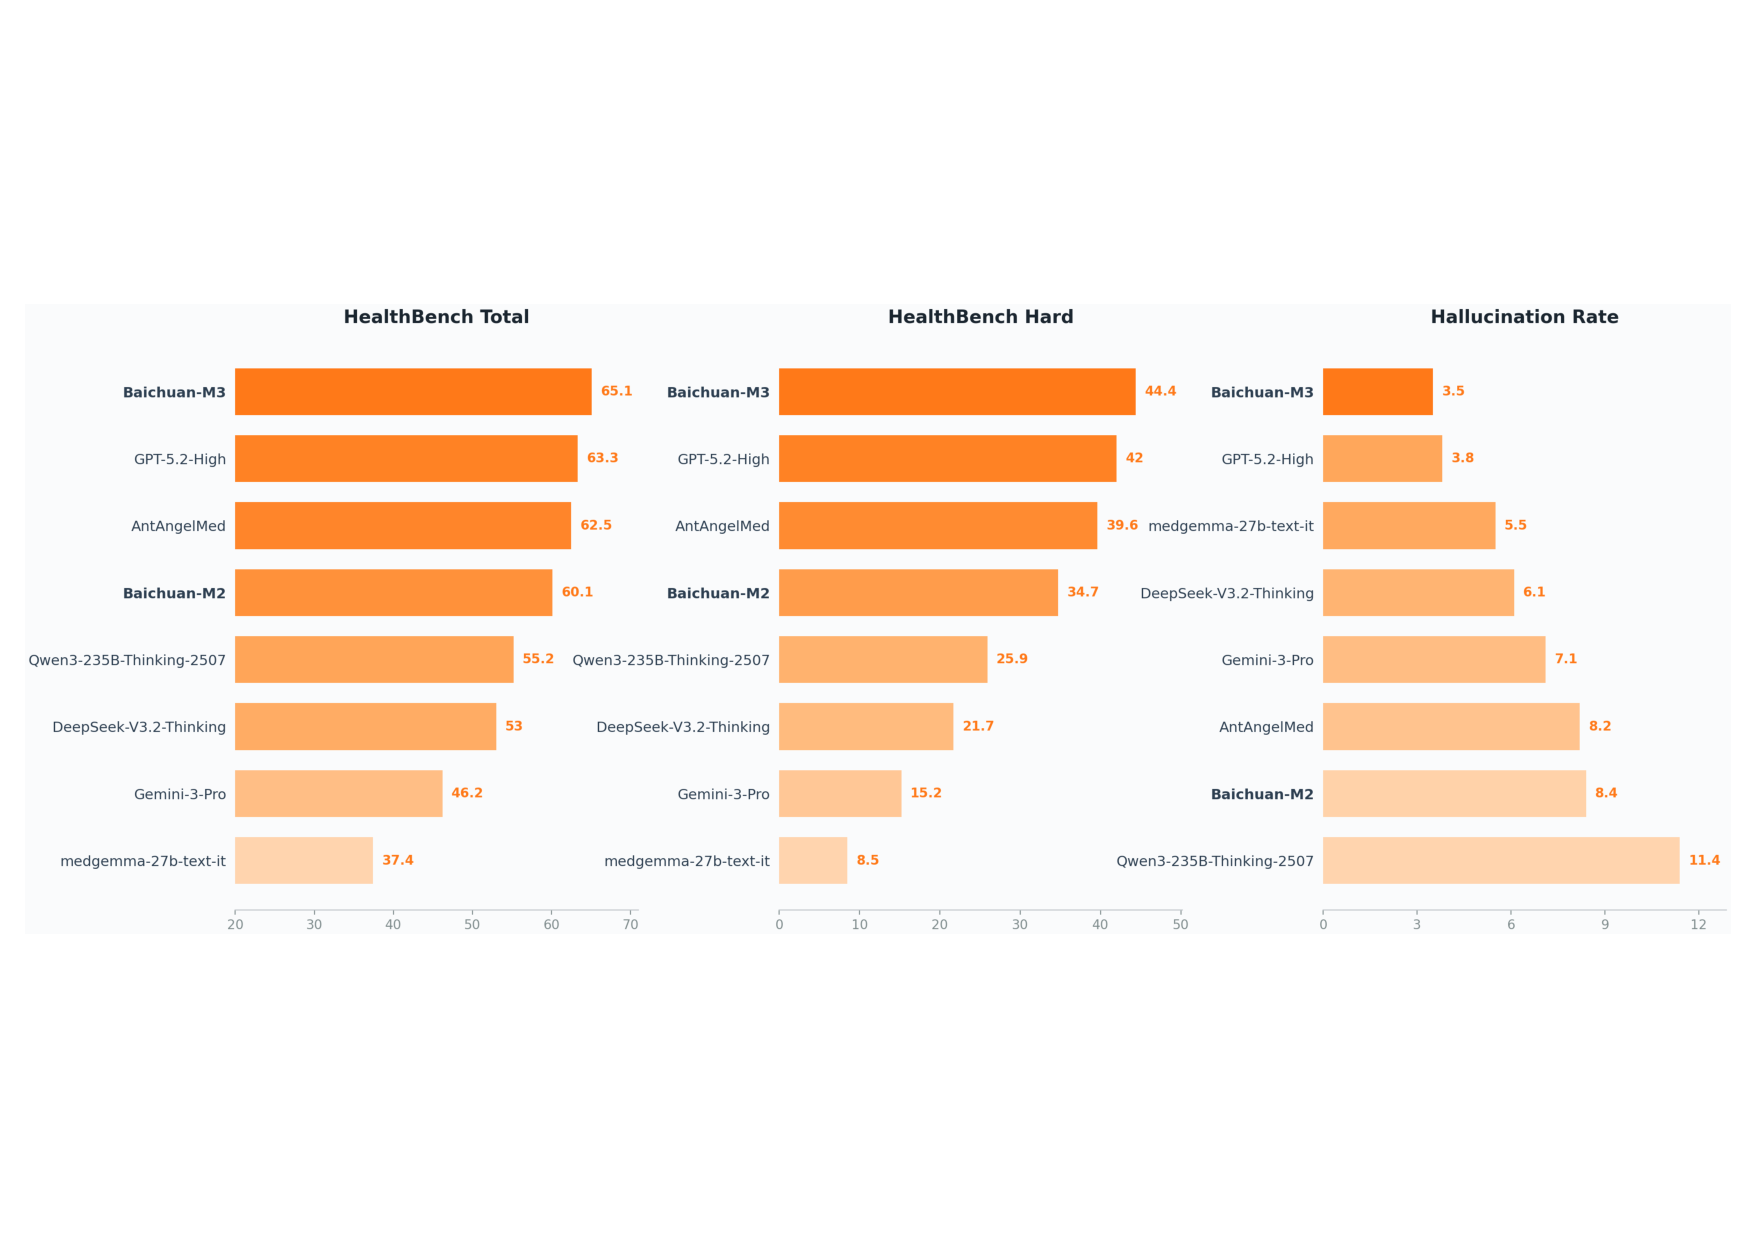
\includegraphics[width=0.98\linewidth]{image/healthbench.pdf}
    \caption{HealthBench 总体性能对比。}
    \label{fig:exp_hb}
\end{figure}

% 3. 第二段：Fine-grained Analysis (M2 vs M3 对比)
与 M2 相比，M3 在大多数评估维度上均有广泛提升，从而形成更稳健、均衡的医疗服务能力画像（见图~\ref{fig:hb_m2_m3}）。提升尤以“上下文寻求”与“上下文感知”为显著。我们将这些增益归因于深度临床问诊训练的迁移：M3 更主动地补充缺失病史与风险因素，同时能够识别影响临床决策的上下文约束。因此，它生成的治疗建议与分诊评估更完整可靠。总体而言，这些结果表明 M3 将问诊任务中学到的“问诊—澄清—决策”交互范式泛化到了更广泛的医疗场景。

\begin{figure}[t]
    \centering
    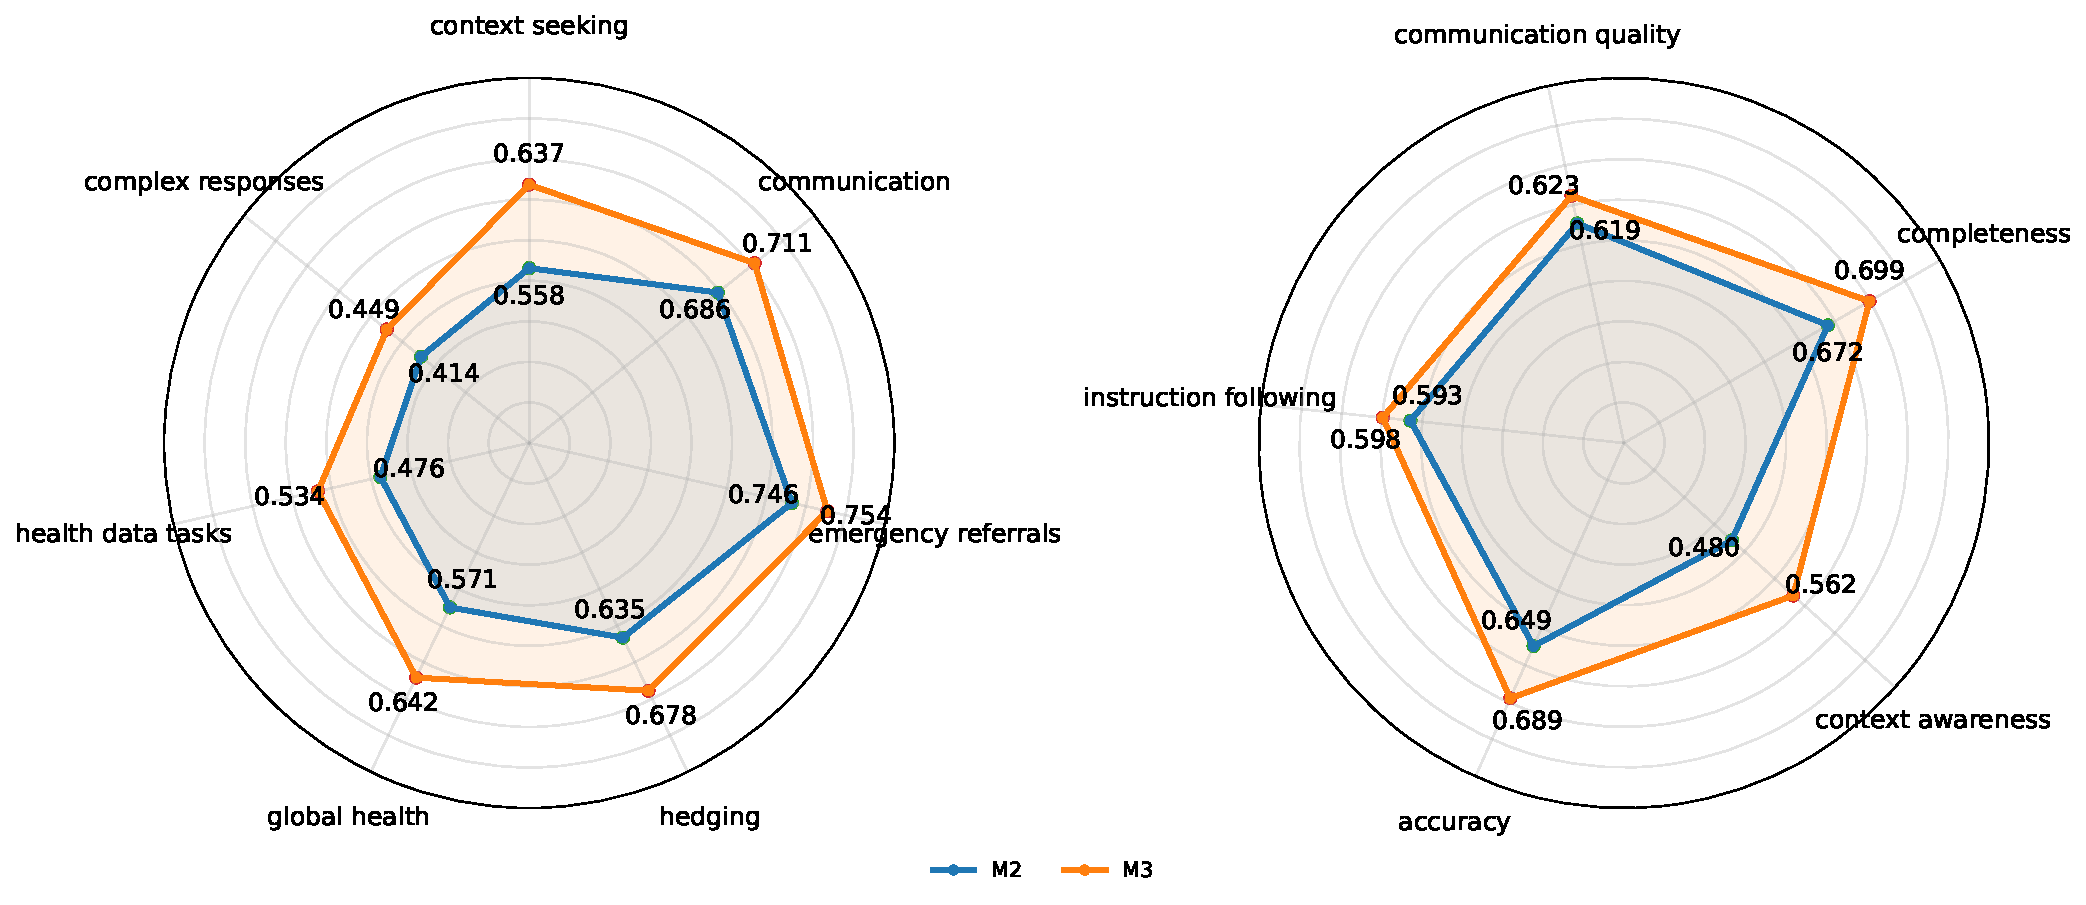
\includegraphics[width=1.0\linewidth]{image/healthbench_radar_m2_vs_m3.pdf}
    \caption{HealthBench fine-grained comparison: M2 vs M3 (themes \& axes).}
    \label{fig:hb_m2_m3}
\end{figure}


% \subsubsection{HB-hard}

\subsubsection{HealthBench-Hallu}

尽管 HealthBench 等基准已为医学 LLM 评估建立了标准，临床安全性仍是医疗 AI 落地的首要考虑。医学幻觉指生成表面合理但事实错误的信息，这一问题已被监管机构与研究社区广泛关注~\cite{ankit2023medhalt, DBLP:journals/corr/abs-2503-05777, DBLP:conf/bionlp/ManesRCBHS24}。该问题在复杂医学推理任务中尤为突出：模型输出通常包含高信息密度的长文本，涵盖精确药物剂量、罕见临床表现等专业知识。长文本生成与语言连贯性相结合，使细粒度事实错误更易逃逸检测，从而带来显著临床风险。因此我们提出 HealthBench-Hallu，一个细粒度评估框架，用于衡量模型在 HealthBench 任务中的事实完整性。该指标通过将输出拆解为原子事实并与外部证据核验，对医学幻觉进行严格量化。


\paragraph{指标设计}

HealthBench-Hallu 关注模型生成内容中的医学事实误解，主要表现为：

\begin{itemize}
    \item \textbf{错误或误用的医学知识：} 叙述错误的临床事实，或将正确知识应用于不恰当语境。
    \item \textbf{伪造或扭曲的医学证据：} 虚构不存在的参考资料、篡改临床数据或捏造因果关系。
\end{itemize}


\paragraph{HealthBench-Hallu 评估}
HealthBench-Hallu 复用事实感知验证流水线（见第~\ref{sec:fact-verifier} 节），但以高精度（而非高吞吐）配置运行：将事实抽取器升级为 GPT-5 以提升细粒度原子事实覆盖，并执行实时多轮检索验证，而非依赖缓存证据。
基于该验证流水线生成的证据标签，我们计算加权幻觉率（$H$）：

\begin{equation}
H = \frac{\sum_{i=1}^{N} w_i}{|\text{Total Claims}|}
\end{equation}

权重 $w_i$ 依据事实风险分层：\textbf{Refuted}（1.0）代表严重事实错误；\textbf{Uncertain}（0.5）代表证据不足或存在歧义风险的陈述；\textbf{Supported}（0.0）代表正确陈述。该指标直接反映模型在复杂医学问题上的可信边界。


\paragraph{实验结果}

表~\ref{tab:hallu_vs_cap} 显示，融合事实感知 RL 使 Baichuan-M3-235B 能够在保留医学推理能力的同时有效抑制幻觉。模型在任务表现上保持竞争力（HealthBench 得分 65.1，与无 RL 变体的 66.2 接近），同时将“被证伪率”和“不确定率”均显著降低约 50\%。这些结果表明，自适应加权策略有效缓解了安全约束与模型效用之间的典型权衡，避免了过度保守方法常见的推理退化。

\begin{table}[htbp]
  \centering
  \caption{Trade-off between hallucination suppression and capability}
    \begin{tabular}{lccc}
    \toprule
    \multicolumn{1}{c}{\textbf{Model}} & \textbf{HealthBench Score} & \textbf{Refuted Rate} & \textbf{Uncertain Rate} \\
    \midrule
    GPT-5.2-High & 63.3  & 2.37\% & 2.78\% \\
    Baichuan-M2-32B & 60.1  & 5.73\% & 5.43\% \\
    M3 - w/o Fact Aware RL & 66.2  & 4.68\% & 3.64\% \\
    \textbf{Baichuan-M3-235B} & \textbf{65.1} & \textbf{2.45\%} & \textbf{2.07\%} \\
    \bottomrule
    \end{tabular}%
  \label{tab:hallu_vs_cap}%
\end{table}%

\paragraph{通过知识探针的幻觉分析}

为阐明事实感知 RL 降低幻觉率的内在机制，我们使用知识探针对模型的\textit{内部认知}（参数化真值）与\textit{外部输出}（生成事实）的一致性进行分析，如图~\ref{fig:Knowledge_Boundary_Alignment} 所示。该分析可通过判断输出是否忠实反映内部参数或因生成不稳定而偏离，从而解耦错误来源。

\begin{figure}[h]
    \centering
    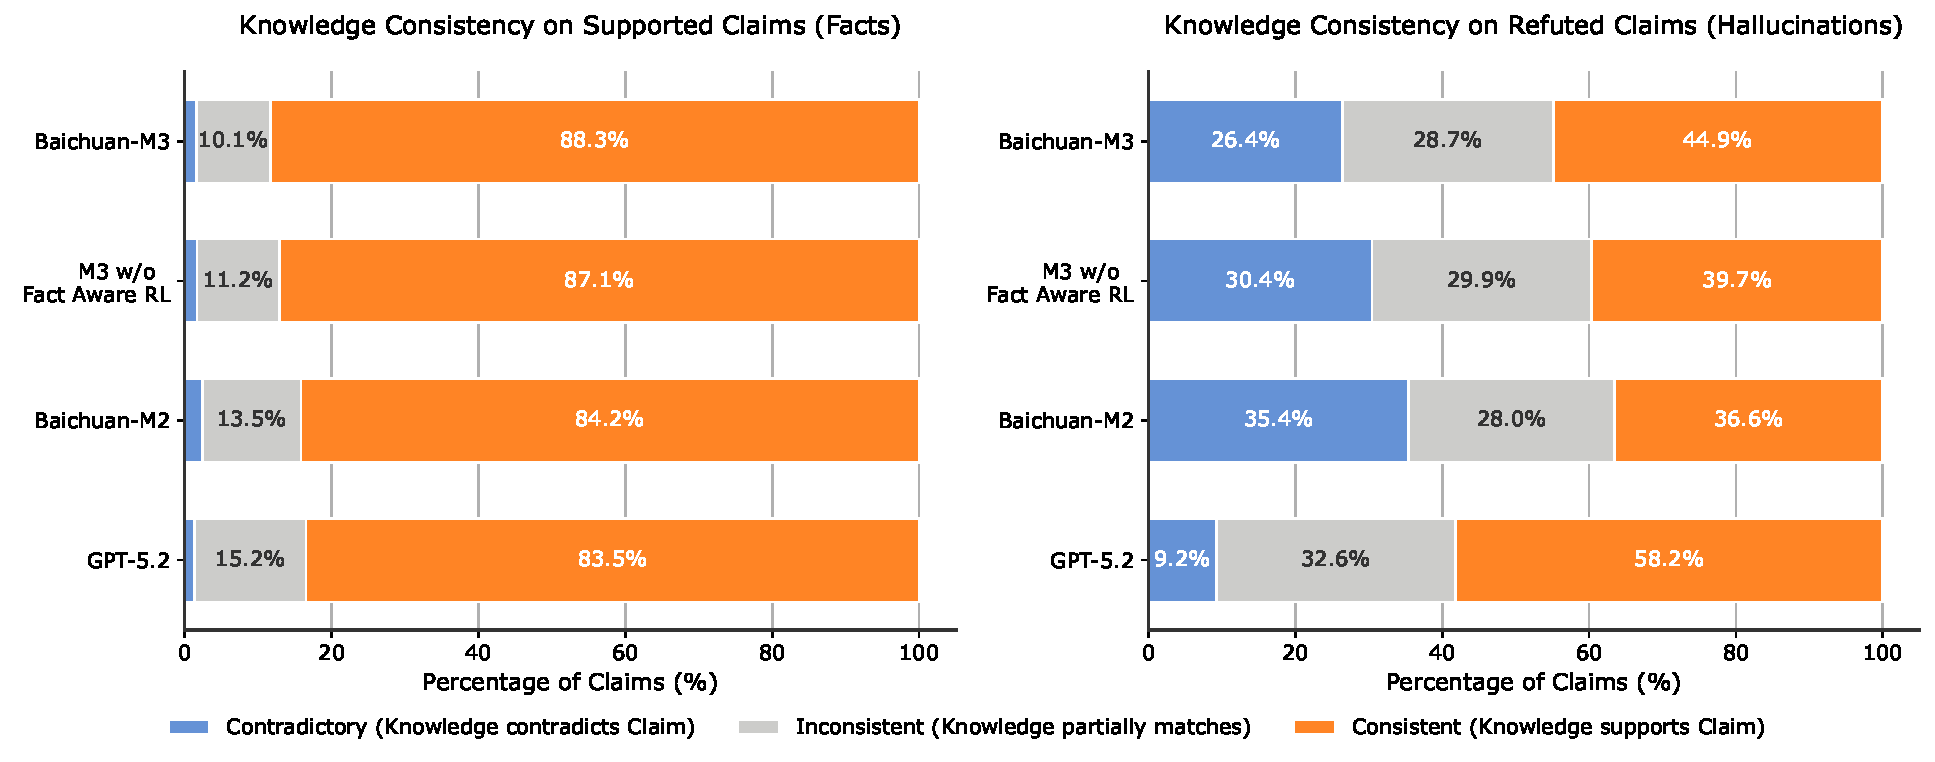
\includegraphics[width=0.98\linewidth]{image/Knowledge_Boundary_Alignment.pdf}
    \caption{\textbf{知识边界一致性分析。} 我们将内部参数与生成事实的一致性划分为三种状态：\textit{一致}（输出与内部认知一致）、\textit{不一致}（部分不匹配）与\textit{矛盾}（输出与内部认知相反）。注意，在幻觉（被证伪事实）情境下，“一致”意味着源于内部知识错误的“诚实错误”。}
    \label{fig:Knowledge_Boundary_Alignment}
\end{figure}

结果显示，事实感知 RL 使模型一致性动态出现明显分化。对于事实正确输出（Supported），内部认知与外部输出的一致性保持在 88.3\%，表明模型的事实真值牢固锚定在内部参数中。更关键的是，对于错误输出（Refuted），一致性显著提升至 44.9\%。这一上升意味着“不忠实幻觉”显著减少——即模型内部认知正确却生成相反错误信息的情形。数据表明剩余幻觉主要是\textit{诚实错误}，即外部输出忠实反映了模型参数中的误解。

最终，这些发现表明事实感知 RL 的主要作用不在于注入新知识，而在于约束模型生成策略，使其严格收敛于自身真实的知识边界内。



\section{推理优化}
% xudong
为提升 Baichuan-M3 在医疗应用中的可用性与高效部署，我们实施了两类推理优化策略。
首先，为加速文本生成，引入 Gated Eagle-3 推测解码方法，显著提升推理吞吐。
其次，采用先进量化技术在不损失准确性的前提下降低模型内存需求。
这些推理优化降低了部署门槛，支持先进医学大模型的更广泛应用。


\subsection{推测解码}

推测解码是一种用于自回归生成的推理加速技术。它使用轻量草案模型提出多个候选 token，再由目标模型并行验证。算法接受最长的已验证前缀并丢弃其余候选，使目标模型在每次验证步骤中提交多个 token，从而提升解码吞吐。

在 Eagle-3~\cite{li2025eagle} 框架中，草案模型额外条件化于目标模型的隐状态以利用更丰富的语义信息。然而，目标模型与草案模型之间显著的容量差距可能引发表示失配：高维且信息密集的隐状态可能压垮轻量草案模型，削弱其有效利用辅助信号的能力，导致候选接受率降低，从而限制可达加速比。

为缓解该问题，我们在 Eagle-3 草案模型中引入 Gated-Attention~\cite{qiu2025gated} 模块（称为 Gated Eagle-3；见图~\ref{fig:gated_eagle3}），提供动态可学习的信息注入调节机制。具体而言，注意力输出通过门控单元，并与由当前层输入动态生成的门控向量进行逐元素乘法调制。该设计实现了细粒度、逐维的信息流控制，突出关键特征并抑制冗余或噪声成分。

如附录~\ref{app:eagle_3} 所示，Gated Eagle-3 的平均接受长度提升 0.31，平均吞吐相较 Eagle-3 基线提高 12\%。这些结果表明，对目标模型信息进行选择性调节可更可靠地转化为实际解码加速，并为后续改进提供参考。

\begin{figure}
    \centering
    
\includegraphics[width=1.0\linewidth]{image/gated-eagle3.pdf}
    \caption{Gated Eagle-3 草案模型示意图。}
    \label{fig:gated_eagle3}
\end{figure}



\subsection{量化}
为在资源受限场景下降低 Baichuan-M3 的 GPU 内存占用，我们采用 INT4 权重量化。然而，专家混合（MoE）模型的稀疏激活特性给标准量化校准带来挑战~\cite{DBLP:journals/corr/abs-2503-21135}：校准语料通常只激活部分专家，导致校准偏置。结果是，频繁激活的专家量化准确，而较少激活的专家量化误差更大，可能在推理时引发不稳定且难以预测的精度退化。

为解决该问题，我们提出自生成校准方案以促进专家覆盖的均匀性。具体而言，我们构建多领域提示集合，并使用 BF16 模型生成高质量响应进行校准。该方法具有两点优势：（i）多样提示可激活几乎所有专家，为每个专家提供充足样本，缓解校准偏置；（ii）自生成响应促使量化模型匹配 BF16 模型的输出分布，从而减少分布差异。
量化参数训练基于 AutoRound~\cite{DBLP:conf/emnlp/ChengZSCHLL24} 框架，量化格式遵循 GPTQ~\cite{DBLP:journals/corr/abs-2210-17323} 标准。



实证结果表明，INT4 量化后的 M3 模型在主流基准上相较 BF16 版本实现近乎无损的性能。该结果验证了我们提出的 MoE 专用量化校准策略的有效性，并为大规模稀疏模型部署提供实践指导。

\section{结论}

我们提出 \textbf{Baichuan-M3}，一种将临床问诊与可靠医疗决策统一起来的医学增强型大语言模型。通过显式建模临床工作流程，Baichuan-M3 实现了主动信息获取、连贯的多步推理与有效的幻觉抑制。借助融合任务特定强化学习与多教师蒸馏的三阶段训练范式，模型在事实性与流程型基准（包括 HealthBench、HealthBench-Hallu 与 OSCE 风格的 ScanBench）上取得了优异表现。结果表明，流程对齐的优化是推进临床级医学 LLM 的有效路径。


\section{局限与未来工作}

Baichuan-M3 目前主要适用于离散的、基于文本的临床场景，尚无法完整覆盖纵向病程管理、多模态临床信号或跨患者轨迹的超长时程推理。尽管幻觉控制已显著提升，但罕见高风险错误与对循证来源的显式扎根仍是开放挑战。未来工作将聚焦于将模型扩展至全路径临床推理，支持多模态输入、长上下文优化，并更紧密地融合证据检索、安全约束与环境驱动的强化学习。


\section{贡献}

贡献者按名字首字母顺序排列。星号（*）表示已不在团队中的成员。

\subsection*{核心贡献者}

Chengfeng Dou, 
Fan Yang, 
Fei Li, 
Jiyuan Jia, 
Qiang Ju, 
Shuai Wang, 
Tianpeng Li, 
Xiangrong Zeng*, 
Yijie Zhou

\subsection*{贡献者}

Hongda Zhang, 
Jinyang Tai, 
Linzhuang Sun, 
Peidong Guo, 
Yichuan Mo

\subsection*{专家与顾问}

Xiaochuan Wang,
Hengfu Cui, 
Zhishou Zhang


\printbibliography[heading=bibintoc, title={参考文献}]

\newpage
\appendix
\section{附录}
本附录给出补充实验结果与详细分析，以进一步验证我们提出的方法。具体而言，我们提供 SPAR 算法与 Clip-Forward-KL 目标的消融实验，并扩展评估事实感知 RL 框架与 Gated Eagle-3 推测解码机制。有关训练与评估所使用提示词的完整细节，请参阅对应的 \href{https://github.com/baichuan-inc/Baichuan-M3-235B/tree/main/prompts}{GitHub} 仓库。

\subsection{SPAR 的消融实验}

\begin{figure}[H]
    \centering
   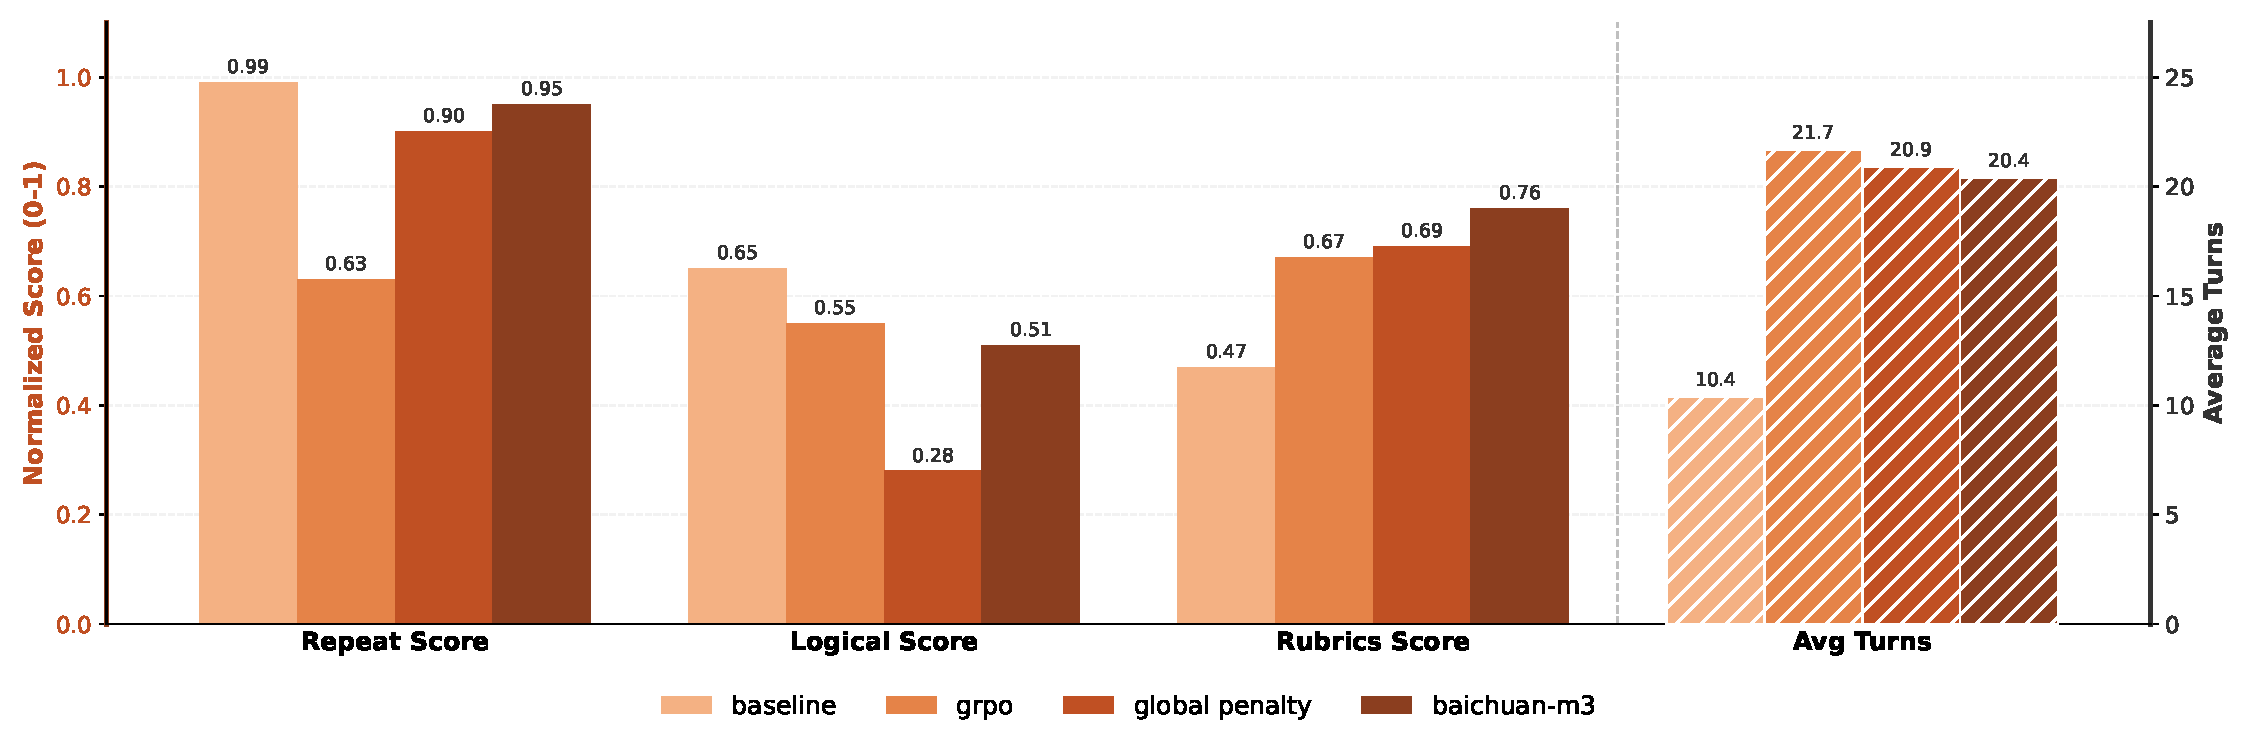
\includegraphics[width=0.98\linewidth]{image/SPAR.pdf}
    \caption{多轮医学问诊任务中 SPAR 与基线模型的性能对比。}
    \label{fig:SPAR}
\end{figure}

为系统评估 SPAR 算法在多轮医学问诊任务中的有效性，我们采用以下实验配置进行消融：
\begin{enumerate}
\item \textbf{Backbone：} 使用 Baichuan-M3 基座模型（RL 之前）作为基础架构。

\item \textbf{GRPO（全局奖励）：} 采用 GRPO 算法，仅使用基于最终问诊结果的全局奖励，不包含中间反馈。

\item \textbf{全局惩罚：} 在 GRPO 基线上引入全局重复惩罚以减轻对话冗余。

\item \textbf{SPAR（Baichuan-M3）：} 实现所提出的逐步奖励计算算法，提供细粒度指导。
\end{enumerate}

\textbf{指标：} 评估框架包含四项归一化到 $[0, 1]$ 区间的指标：重复评分（衡量非冗余）、逻辑评分、量表评分与平均轮次（Avg Turns）。其中前两项通过 GPT-5 对对话日志进行三档打分 $(0, 1, 2)$ 并归一化得到。

\textbf{结果：} 如图~\ref{fig:SPAR} 所示，仅使用全局奖励的 GRPO 训练虽能稳步提升量表评分，但也增加了冗余问询（重复评分下降）。加入全局重复惩罚可有效降低冗余，却导致逻辑评分显著下降，表明逻辑碎片化严重。这表明粗粒度全局惩罚会显著扰动模型的自然推理流程。相比之下，SPAR 取得更好的平衡：显著减少重复同时保持逻辑连贯。该双重优化使模型在有限问诊轮次中提取更高密度的关键医学信息。



\subsection{事实感知 RL} 
\subsubsection{蒸馏事实抽取模型的评估}
\label{sec:extraction_model_evaluation}

离线事实抽取以 GPT-5 作为参考抽取器，但在在线强化学习中部署如此大的教师模型在计算上不可接受。为此，我们通过监督微调（SFT）训练较小模型，以在在线 RL 中充当高效抽取器。我们相对 GPT-5 用三项指标评估抽取保真度：

\begin{itemize}
    \item \textbf{召回率：} 衡量 SFT 模型相对参考基线（GPT-5）的覆盖程度。
    \item \textbf{SFT 独有率：} SFT 模型识别但 GPT-5 未识别的事实占比，反映潜在过度生成或新信息发现。
    \item \textbf{GPT 独有率：} GPT-5 识别但 SFT 模型未捕获的事实占比，反映信息丢失。
\end{itemize}

\begin{table}[H]
\centering
\caption{不同规模事实抽取模型的对比实验。}
\label{tab:model_performance}
\begin{tabular}{lcccc}
\toprule
Model & Recall (\%) & Our Exclusive Rate (\%) & GPT Exclusive Rate (\%) & Claim Count \\
\midrule
Qwen3-8B & 30.45 & 31.02 & 69.55 & 8.50 \\
Qwen3-32B & 37.68 & 33.29 & 62.32 & 12.81 \\
SFT-A3B-30B & 69.69 & 46.89 & 30.31 & 47.19 \\
SFT-8B & 72.80 & 45.60 & \textbf{27.20} & 46.66 \\
SFT-32B & \textbf{73.00} & 47.15 & \textbf{27.01} & \textbf{46.78} \\
\bottomrule
\end{tabular}
\end{table}

如表~\ref{tab:model_performance} 所示，SFT 显著提升抽取性能，8B 模型召回率达到 72.80\%，而未微调基线仅为 30.45\%。尽管 32B 版本带来边际提升，但其部署成本过高，不适合在线 RL 流水线。我们最终采用 SFT-8B 作为事实抽取器，在保真度与部署约束之间取得平衡。

\subsubsection{奖励组件消融}
\label{sec:ablation_reward}

我们从一个中间 SFT 检查点出发，对不同奖励塑形策略的影响进行比较：一是仅优化任务奖励的 \textit{w/o Fact Aware RL} 模型，二是使用式~\eqref{eq:naive-objective} 中静态幻觉惩罚的 \textit{Baseline}。

\begin{figure}[H]
    \centering
    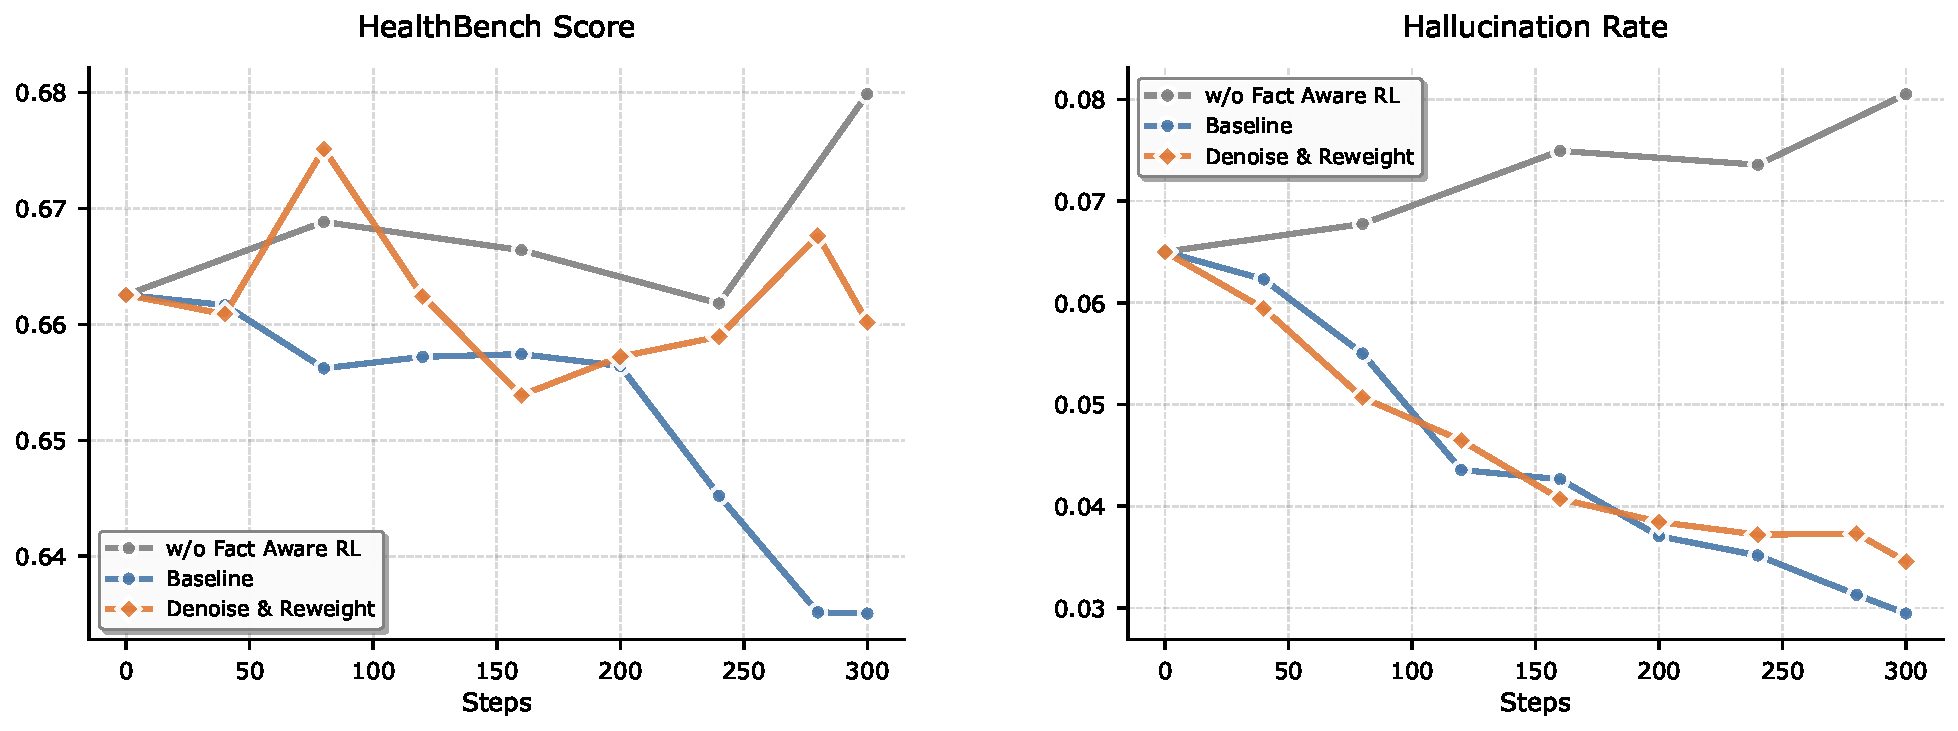
\includegraphics[width=0.98\linewidth]{image/fact-aware-rl-ablation.pdf}
    \caption{不同优化策略的训练动态。图中对比各目标对医学推理能力（左）与事实可靠性（右）的影响。}
    \label{fig:training_dynamics}
\end{figure}

图 \ref{fig:training_dynamics} 展示了不同目标驱动的行为差异。\textit{w/o Fact Aware RL}（灰色）取得最高 HealthBench 得分（约 0.68），但出现明显幻觉漂移（上升到 0.08）。这说明不受约束的优化目标倾向于推动模型生成更长内容，从而削弱事实稳定性。\textit{Baseline}（蓝色）虽纠正了漂移，却过度补偿；其激进的幻觉抑制导致推理能力严重退化，体现惩罚诱导的保守性。

我们在式~\eqref{eq:full-fact-aware-rl} 中提出的 \textit{去噪与重加权} 策略有效将安全对齐与能力损失解耦：其幻觉率降低到约 0.035，与 Baseline 相当，同时推理得分（约 0.665）接近无约束模型起点。这一稳定性验证了双重保护设计的有效性，即边际噪声过滤与能力门控协同工作。因此，该方法在保持核心医学效用的同时，引导模型走向事实正确性。

\subsection{离线专家融合中 Clip-Forward-KL 的消融}
\label{sec:ablation_clip_fkl}

我们分析 Clip-Forward-KL 在离线专家融合中的作用。
学生模型从\textit{医学问诊专家}初始化，并通过离线蒸馏融合\textit{健康咨询专家}。
在相同初始化、数据集与训练配置下，问诊与健康咨询数据分别采用 Clip-Forward-KL 或标准 Forward-KL 进行蒸馏。

表~\ref{tab:clip_ablation} 报告了 ScanBench、HealthBench 与 HealthBench-Hard 的结果。
ScanBench 主要反映医学问诊能力的保留，
而 HealthBench 与 HealthBench-Hard 评估更广泛医疗知识的融合效果。

\begin{table}[H]
\centering
\caption{离线专家融合中 Clip-Forward-KL 的消融。
在相同训练配置下，Clip-Forward-KL 提升 HealthBench 与 HealthBench-Hard，同时保持与 ScanBench 相当的性能。}
\label{tab:clip_ablation}
\begin{tabular}{lccc}
\toprule
Method & ScanBench & HealthBench & HealthBench-Hard \\
\midrule
Forward-KL & 73.7 & 58.6 & 33.2 \\
Clip-Forward-KL & 73.5 & \textbf{61.1} & \textbf{38.5} \\
\bottomrule
\end{tabular}
\end{table}

Clip-Forward-KL 在保持问诊性能的同时显著提升医疗基准，表明其更有效地融合了新领域知识。
这说明标准 Forward-KL 往往会在稀疏离线样本上过度放大概率，从而干扰新医疗能力的融合而非保留既有问诊能力。
通过对教师支持动作施加单侧下界约束，Clip-Forward-KL 实现更保守的融合，并为在线优化提供良好初始化。

\subsection{Gated Eagle-3 推测解码的消融实验}

为保证严格且公平的比较，我们在相同的 35,000 条训练样本与训练协议下，对原始 Eagle-3 草案模型与我们提出的 Gated Eagle-3 进行评估。两者在统一推理配置下覆盖 GSM8K~\cite{DBLP:journals/corr/abs-2110-14168}、HumanEval~\cite{DBLP:journals/corr/abs-2107-03374}、MT-Bench~\cite{DBLP:conf/nips/ZhengC00WZL0LXZ23} 和 HealthBench 等代表性基准。所有实验在 NVIDIA H20 GPU 上进行，模型训练使用 SpecForge~\cite{specforge2025} 框架，推理通过 SGLang~\cite{zheng2024sglang} 执行。如表~\ref{tab:eagle_comparison} 所示，Gated Eagle-3 相比 Eagle-3 基线的平均接受长度提升 0.31。
此外，在并行度为 8 的设置下，吞吐对比如表~\ref{app:eagle_throughput_comparison} 所示。

\label{app:eagle_3}
\begin{table}[H]
\centering
\caption{Eagle-3 基线与 Gated Eagle-3 的平均接受长度对比。}
\label{tab:eagle_comparison}
\begin{tabular}{lcccc}
\toprule
Method & GSM8K & HumanEval & MT-Bench & HealthBench  \\
\midrule
Eagle-3 Base & 3.59 & 3.58 & 2.97 & 2.41 \\
Gated Eagle-3  & \textbf{3.84} & \textbf{4.03} & \textbf{3.23} & \textbf{2.70}  \\
\midrule
$\Delta$ (Gain) & +0.25 & +0.45 & +0.26 & +0.29  \\
\bottomrule
\end{tabular}
\end{table}

\begin{table}[H]
\centering
\caption{Eagle-3 基线与 Gated Eagle-3 的吞吐对比（tokens/s）。}
\label{app:eagle_throughput_comparison}
\begin{tabular}{lcccc}
\toprule
Method & GSM8K & HumanEval & MT-Bench & HealthBench  \\
\midrule
Eagle-3 Base & 376.98 & 576.19 & 451.39 & 356.94  \\
Gated Eagle-3 & \textbf{431.26} & \textbf{646.17} & \textbf{490.12} & \textbf{400.52}  \\
\midrule
$\Delta$ (Gain) & +14.40\% & +12.15\% & +8.58\% & +12.21\%  \\
\bottomrule
\end{tabular}
\end{table}



%\appendixpage

\addappheadtotoc

\end{document}